\documentclass[11pt,a4paper]{article}

% ------------------------------------------------
% PACKAGES
% ------------------------------------------------
\usepackage[a4paper,margin=2.25cm]{geometry}
\usepackage[english]{babel}
\usepackage[T1]{fontenc}
\usepackage{lmodern}
\usepackage{amsmath}
\usepackage{amssymb}
\usepackage{graphicx}
\graphicspath{{images/}}
\usepackage{booktabs}
\usepackage{array}
\usepackage{enumitem}
\usepackage{xurl}
\usepackage{xcolor}
\usepackage{listings}
\usepackage[hidelinks]{hyperref}
\usepackage{float}
\usepackage{caption}

% ------------------------------------------------
% DOCUMENT FORMATTING
% ------------------------------------------------
\setlength{\parskip}{0.45em}
\setlength{\parindent}{0pt}

\setlist[itemize]{
    topsep=3pt,
    itemsep=2pt,
    leftmargin=1.5em
}

\setlist[enumerate]{
    topsep=3pt,
    itemsep=3pt,
    leftmargin=1.8em
}

\renewcommand{\arraystretch}{1.2}


% Compact embedded figures: preserve aspect ratio and avoid oversized images.
\newcommand{\reportimage}[2]{%
\begin{figure}[H]
    \centering
    \includegraphics[width=0.72\linewidth,height=0.42\textheight,keepaspectratio]{#1}
    \caption{#2}
    \label{fig:#1}
\end{figure}%
}

% A compact resource link; internal figure references remain separate.
\newcommand{\resourcelink}[2]{\noindent\textbf{#1:} \href{#2}{Open link}\par}

% ------------------------------------------------
% CODE PATH BOX
% ------------------------------------------------
\newcommand{\codepath}[1]{%
    \begin{center}
        \fbox{\parbox{0.88\linewidth}{\centering\ttfamily\small\detokenize{#1}}}
    \end{center}%
}

% ------------------------------------------------
% FIGURE PLACEHOLDER
% ------------------------------------------------
\newcommand{\placeholderfigure}[2]{
\begin{figure}[H]
    \centering
    \fbox{
        \parbox[c][4.0cm][c]{0.88\textwidth}{
            \centering
            \textbf{#1}\\[0.6em]
            #2
        }
    }
    \caption{#1}
\end{figure}
}

% ------------------------------------------------
% TWO FIGURES SIDE BY SIDE
% ------------------------------------------------
\newcommand{\placeholderpair}[4]{
\begin{figure}[H]
    \centering
    \begin{minipage}{0.47\textwidth}
        \centering
        \fbox{
            \parbox[c][3.2cm][c]{0.92\linewidth}{
                \centering
                \textbf{#1}\\[0.5em]
                #2
            }
        }
    \end{minipage}
    \hfill
    \begin{minipage}{0.47\textwidth}
        \centering
        \fbox{
            \parbox[c][3.2cm][c]{0.92\linewidth}{
                \centering
                \textbf{#3}\\[0.5em]
                #4
            }
        }
    \end{minipage}
\end{figure}
}

% ------------------------------------------------
% DOCUMENT
% ------------------------------------------------
\begin{document}

% =================================================
% TITLE PAGE
% =================================================

\begin{titlepage}
    \centering

    \vspace*{2.2cm}

    {\Huge\bfseries Progress Log\par}

    \vspace{1.0cm}

    {\Large Wi-Fi-Controlled Unmanned Ground Vehicle\par}

    \vspace{1.8cm}

    {\large\textbf{Prepared by}\par}

    \vspace{0.4cm}

    {\large
    Nehan Mohammad\\[0.25em]
    T. Pranay Siddarth Reddy\\[0.25em]
    Akshit
    \par}

    \vfill

    {\large
    \textbf{Assigned by}\\
    Prof. Dr. GVV Sharma
    \par}

    \vspace*{1.3cm}

\end{titlepage}


% =================================================
% ACKNOWLEDGMENT
% =================================================

\section*{Acknowledgment}
\addcontentsline{toc}{section}{Acknowledgment}

We would like to thank Prof. Dr. GVV Sharma for assigning
this project and giving us the opportunity to work on a
practical wireless-control system.

The project involved combining circuit design, embedded
programming, motor control, and wireless communication.
The practical work helped us understand the challenges
involved in developing a reliable physical system.

This document records the models explored, the progress
made during development, the problems encountered, and
the possible future extensions of the project.

Photographs, circuit diagrams, interface screenshots,
source-code locations, and demonstration links are
included wherever applicable.


% =================================================
% TABLE OF CONTENTS
% =================================================

\newpage

\setcounter{tocdepth}{3}
\tableofcontents

\newpage

\listoffigures

\newpage


% #################################################
% SECTION 1: PROGRESS LOG
% #################################################

\section{Progress Log}

This section records the development of the UGV in
chronological order. It describes the work carried out
during each stage, the hardware and software used,
the problems encountered, and the changes made during
development.

The detailed technical descriptions of the models are
provided separately in Section~\ref{sec:project-models}.
Clickable references are included at the end of each
day's entry.


% -------------------------------------------------
% DAY 1
% -------------------------------------------------

\subsection{Day 1: Component Collection and Bluetooth Control}

\subsubsection{Component collection}

We began by collecting the main components required
to build the UGV. These included the chassis, two DC
gear motors, an L293D motor driver, an ESP32 DevKit,
connecting wires, and a battery supply.

We reviewed reference material to understand the
general arrangement of the controller, motor driver,
motors, and power supply.

We also prepared a circuit representation in Tinkercad
to plan the connections before proceeding with the
physical assembly.

The reference material included an L298N motor-driver
example, while our actual implementation used the
L293D driver. The reference was therefore used as a
general guide, with the actual connections checked
against our hardware.


\subsubsection{First Bluetooth implementation}

Our first objective was to establish wireless motor
control using an ESP32 DevKit.

We selected the Dabble mobile application because it
provides a Gamepad interface that communicates with
the ESP32 through Bluetooth.

The ESP32 was configured with the Bluetooth device
name \texttt{ESP32\_RC\_Car}. The user connects the
phone to the ESP32, opens the Gamepad interface, and
uses the directional controls to operate the motors.

The ESP32 processes the received inputs and generates
the direction and PWM signals required by the L293D
motor driver.

The initial Bluetooth implementation successfully
demonstrated wireless control of the rover.


\subsubsection{Problems encountered}

A few practical problems appeared during the initial
assembly and testing.

\begin{itemize}

    \item \textbf{Improper motor soldering:}
    Some motor connections were not soldered properly.
    This was resolved by reworking and resoldering
    the affected connections.

    \item \textbf{Loose jumper-wire connections:}
    Several connections were not sufficiently secure,
    causing intermittent contact. This remained a
    recurring issue during later testing.

    \item \textbf{Power stability:}
    During later Wi-Fi experiments, the ESP32 did not
    behave reliably. We suspected that the power
    arrangement might have contributed, but did not
    establish a single confirmed cause.

\end{itemize}


\subsubsection{Outcome}

The ESP32 DevKit successfully operated the initial
Bluetooth-controlled rover.

This model established the basic wireless motor-control
approach that was later extended through browser-based
Wi-Fi control.

The detailed implementation is described in
\hyperref[model:bluetooth]{Model 1: Bluetooth Control
Using Dabble (Section~\ref*{model:bluetooth})}.


% -------------------------------------------------
% DAY 2
% -------------------------------------------------

\newpage

\subsection{Day 2: Local Wi-Fi Joystick Control (Main Project)}

\subsubsection{Transition to Wi-Fi control}

After developing the Bluetooth-controlled model, we
wanted to explore a browser-based interface for
operating the rover.

The objective was to create a local Wi-Fi network
using the microcontroller itself. A phone or laptop
could connect to this network and control the rover
through a webpage.

We initially attempted an ESP32-based Wi-Fi setup.
However, its operation was not sufficiently reliable
during testing. We also experimented with a NodeMCU
board, but the issue persisted.

To continue development, we shifted the local Wi-Fi
implementation to a Raspberry Pi Pico W.


\subsubsection{Pico W local network}

The Raspberry Pi Pico W was configured to create its
own wireless access point with the network name
\texttt{UGV}.

A phone or laptop can connect directly to this network
without requiring an external router or campus Wi-Fi.

After connecting, the user opens the control webpage
through the browser at:

\begin{center}
    \texttt{http://192.168.4.1}
\end{center}

The webpage provides a virtual joystick. Its horizontal
and vertical values are transmitted to the Pico W
through HTTP requests.

The controller processes these values and generates
the corresponding motor commands using differential
drive.


\subsubsection{Multi-device connectivity}

One of the important advantages of the local Wi-Fi
architecture is that the rover does not have to be
controlled from only one phone or laptop.

The Pico W access point supports up to four connected
Wi-Fi clients simultaneously. Therefore, multiple
devices can join the \texttt{UGV} network and access
the browser-based control interface at the same time.

This provides a useful multi-device capability:

\begin{itemize}

    \item Multiple phones or laptops can connect to
    the rover's local network.

    \item Each connected device can open the same
    browser-based control webpage.

    \item The control interface does not need to be
    installed separately on every device.

    \item The rover can be accessed locally without
    an internet connection or an external router.

\end{itemize}

The maximum supported access-point client count is
\textbf{4 devices simultaneously}, according to the
Pico W wireless access-point specification.

Since all connected devices communicate with the
same rover, they share the same motor-control system.
Commands received from different devices are processed
by the same controller; a later command can therefore
change the movement requested by an earlier device.

This is shared multi-device access, rather than
independent control of four separate vehicles.

The four-device limit refers to Wi-Fi client
connections, not a guarantee that four simultaneous
high-frequency joystick streams will have identical
response performance.


\subsubsection{Joystick control and stopping behaviour}

The browser interface provides proportional control
rather than only fixed directional commands.

The joystick generates two normalised values:

\begin{itemize}
    \item \(x\): horizontal movement, representing
    left and right steering.
    \item \(y\): vertical movement, representing
    forward and reverse movement.
\end{itemize}

The Pico W combines these values to calculate the
left and right motor commands.

A STOP command is also provided. The firmware uses
a watchdog mechanism to stop the motors if fresh
commands are no longer received.

The browser sends joystick updates at an interval
of 20 milliseconds, corresponding to a nominal
update frequency of 50 Hz.

The watchdog timeout in the documented firmware is
250 milliseconds.


\subsubsection{Campus Wi-Fi distinction}

The Pico W local access-point model is independent
of the campus network. It creates its own network
for direct communication between the phone and rover.

The IITH campus network uses WPA2-Enterprise
authentication. The local Pico W implementation
was not used as a successful campus-network
connection.

This local browser-control model is therefore
separate from the ESP32-CAM campus-network model.


\subsubsection{Outcome}

The Raspberry Pi Pico W successfully provided the
local access-point architecture required for
browser-based control.

The model introduced:

\begin{itemize}
    \item Local Wi-Fi access point named \texttt{UGV}.
    \item Browser-based joystick interface.
    \item HTTP communication with the controller.
    \item Proportional differential-drive control.
    \item PWM-based motor speed control.
    \item Multi-device access for up to four Wi-Fi clients.
    \item STOP command and watchdog-based stopping.
\end{itemize}

The detailed architecture and operation are explained
in
\hyperref[model:wifi]{Model 2: Local Wi-Fi Joystick
Control Using Raspberry Pi Pico W
(Section~\ref*{model:wifi})}.


% -------------------------------------------------
% DAY 3
% -------------------------------------------------

\newpage

Before the Day 3 implementation log, it is worth noting that the ESP32-CAM model was developed almost entirely at the theoretical and design level, including its system architecture, circuit connections, and proposed Wi-Fi-based camera functionality. However, due to component constraints, we were unable to produce the physical model or demonstrate its operation. The theoretical development and implementation plan were completed, providing a foundation for its future physical realization.

\subsection{Day 3: ESP32-CAM Campus Camera Rover}

\subsubsection{Camera-assisted rover concept}

The third stage involved exploring a camera-assisted
rover using an ESP32-CAM board.

The intention was to combine remote rover operation
with a live camera feed. This would allow an operator
to observe the surroundings of the rover while
controlling its movement.

Unlike the local Pico W access-point model, this
approach was intended to use the IITH campus
wireless network.


\subsubsection{Campus network connection}

We successfully established the ESP32-CAM connection
to the IITH campus Wi-Fi network using WPA2-Enterprise
authentication.

This confirmed that the campus-network connection
could be established with the ESP32-CAM.

The remaining difficulty was associated with the
camera hardware and interfacing.


\subsubsection{Camera interfacing problem}

During camera setup, we encountered a hardware or
camera-interfacing problem that prevented successful
camera initialisation.

Although the campus Wi-Fi connection was established,
the camera problem meant that we could not complete
the intended live-streaming demonstration.

The two outcomes are therefore distinct:

\begin{itemize}
    \item ESP32-CAM campus Wi-Fi connection using
    WPA2-Enterprise: successful.
    \item Camera initialisation and live streaming:
    incomplete due to the camera interfacing problem.
\end{itemize}


\subsubsection{Further work}

The next step would be to verify the camera hardware
independently, establish a stable video stream, and
then integrate it with the rover's control interface.

The intended camera rover architecture and the
interfacing issue are discussed in
\hyperref[model:camera]{Model 3: ESP32-CAM Campus
Camera Rover (Section~\ref*{model:camera})}.


% #################################################
% SECTION 2: PROJECT MODELS
% #################################################

\newpage

\section{Project Models}
\label{sec:project-models}

This section describes the three main models explored
during the project. Each model represents a different
approach to wireless control or remote operation
of the UGV.

The models are presented according to their intended
architecture and technical operation. Their practical
development history is recorded separately in the
Progress Log.


% =================================================
% MODEL 1: BLUETOOTH
% =================================================

\subsection{Model 1: Bluetooth Control Using Dabble}
\label{model:bluetooth}

\subsubsection{Objective and system overview}

The first model was developed to establish wireless
control of the UGV through a mobile phone.

An ESP32 DevKit was used as the main controller,
while the Dabble mobile application provided the
user interface.

The application communicates with the ESP32 through
Bluetooth and supplies directional and speed-level
inputs.

The ESP32 processes these inputs and generates the
required direction and PWM signals for the L293D
motor driver.

The overall control sequence is:

\begin{enumerate}
    \item The phone connects to the ESP32 through Bluetooth.
    \item The user opens the Gamepad module in Dabble.
    \item Directional and speed-level inputs are read
    by the ESP32.
    \item The controller calculates the required
    motor commands.
    \item The L293D operates the motors according
    to the received signals.
\end{enumerate}


\subsubsection{Bluetooth connection and Dabble interface}

The Bluetooth device name configured in the firmware
is \texttt{ESP32\_RC\_Car}.

The Dabble application provides a Gamepad interface
through which the user sends directional commands.
The ESP32 reads the relevant button states and
translates them into motor-control values.

The phone supplies the user's input, while the ESP32
performs the control calculations and generates
the signals required by the motor driver.


\begin{figure}[H]
    \centering
    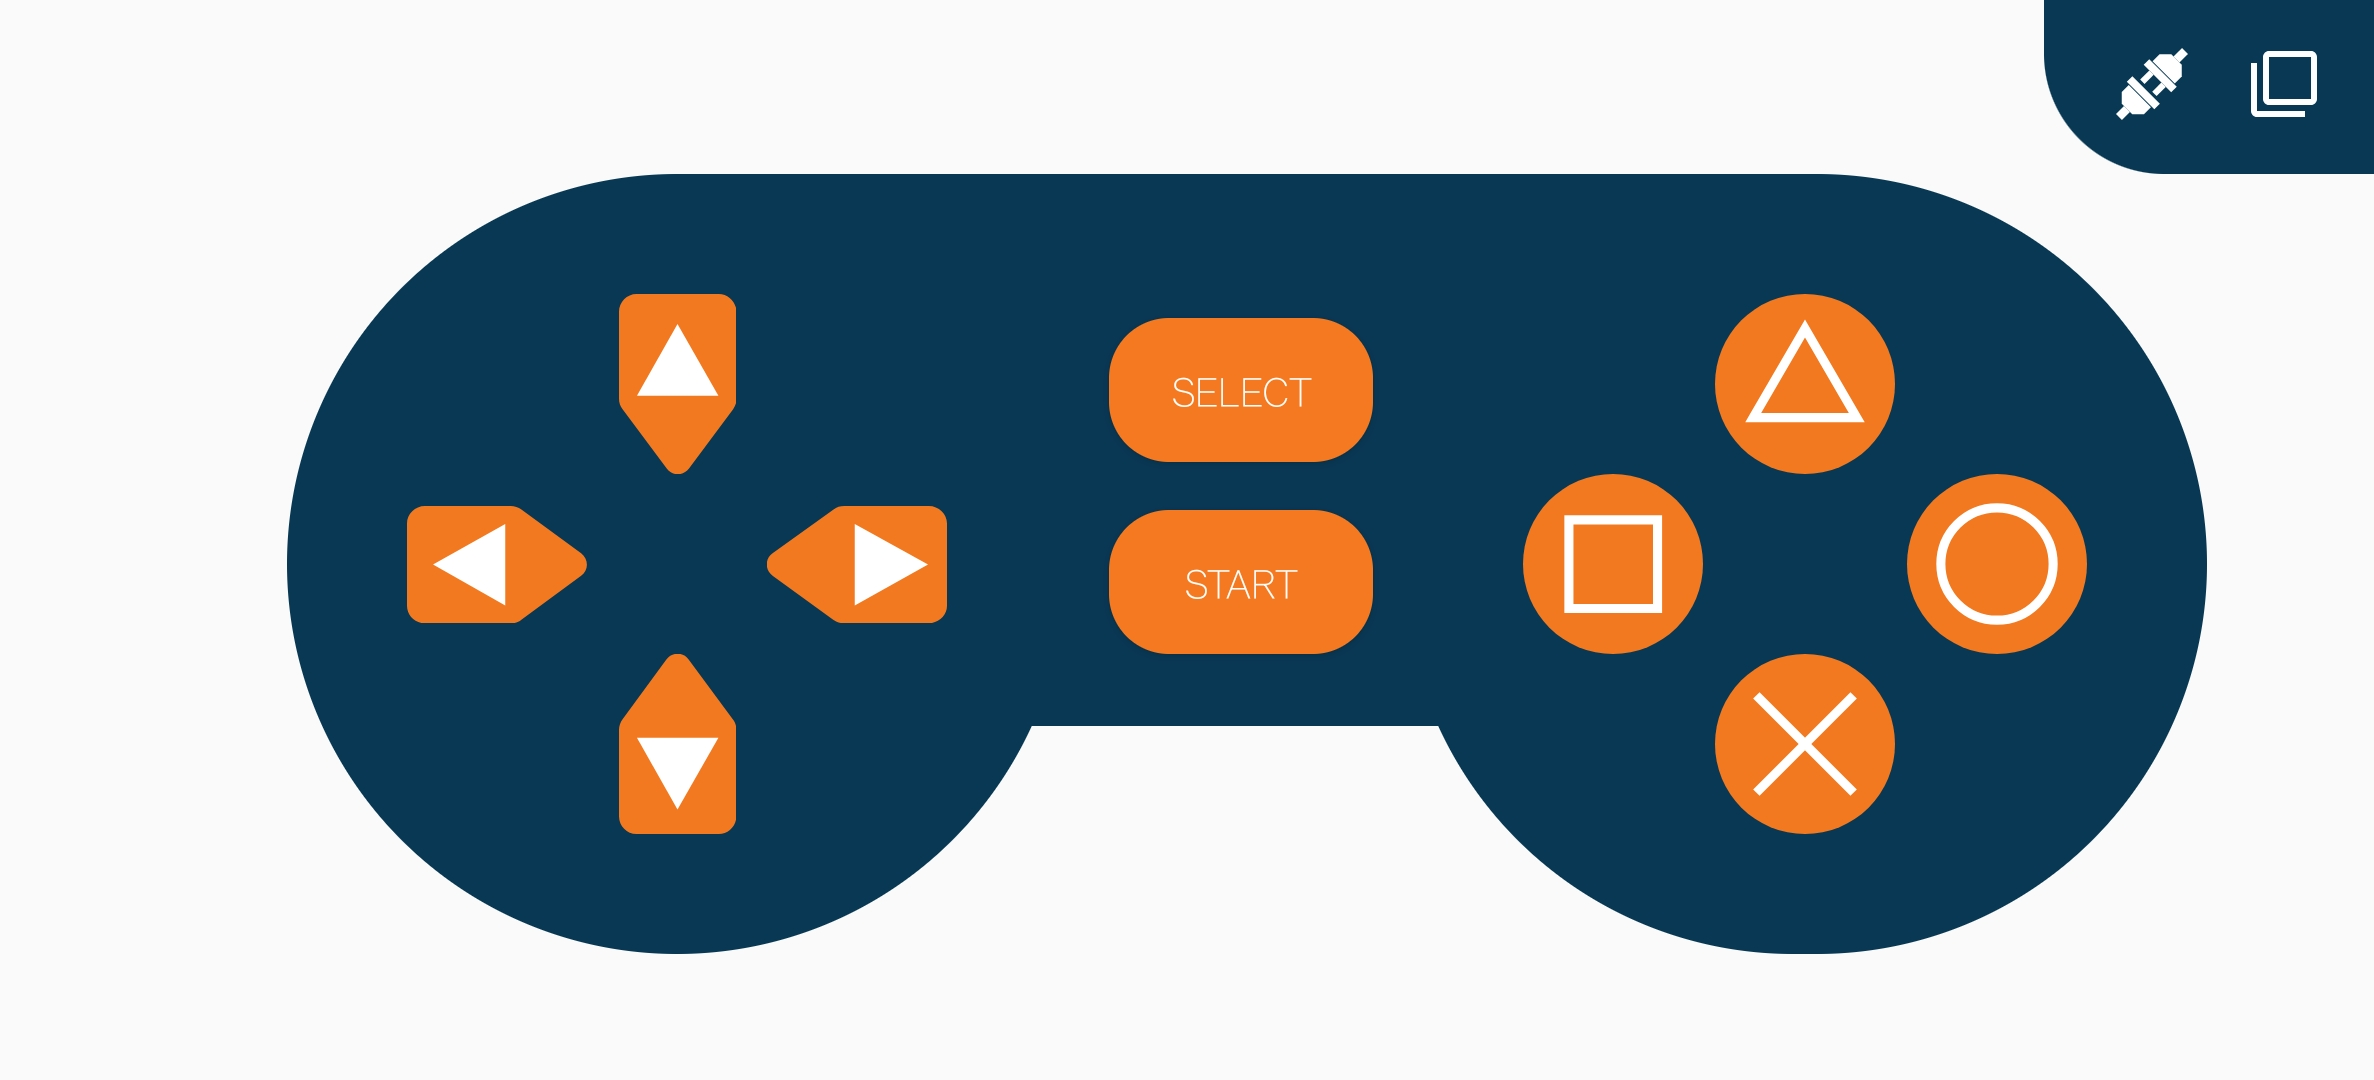
\includegraphics[width=0.70\linewidth,height=0.40\textheight,keepaspectratio]{bluetooth/dabble_gamepad.png}
    \caption{Dabble Gamepad interface used to control the rover.}
    \label{fig:dabble-gamepad}
\end{figure}


\subsubsection{Motor driver and GPIO mapping}

The Bluetooth model uses an L293D motor driver.

The left and right motors have separate direction
inputs and enable signals. The enable pins are used
for PWM-based speed control, while the direction
inputs determine the rotation direction.

\begin{center}
\begin{tabular}{lll}
\toprule
\textbf{Function}
&
\textbf{ESP32 GPIO}
&
\textbf{L293D pin}
\\
\midrule
Left direction input 1 & 32 & 2\\
Left direction input 2 & 33 & 7\\
Left enable / PWM & 27 & 1\\
Right direction input 1 & 25 & 10\\
Right direction input 2 & 26 & 15\\
Right enable / PWM & 14 & 9\\
\bottomrule
\end{tabular}
\end{center}

The right motor is configured with an inversion
setting to account for its physical orientation.
A small right-side trim is also used to compensate
for differences in motor response.


\subsubsection{Circuit diagram}
\label{subsec:bluetooth-circuit}
\begin{figure}[H]
    \centering
    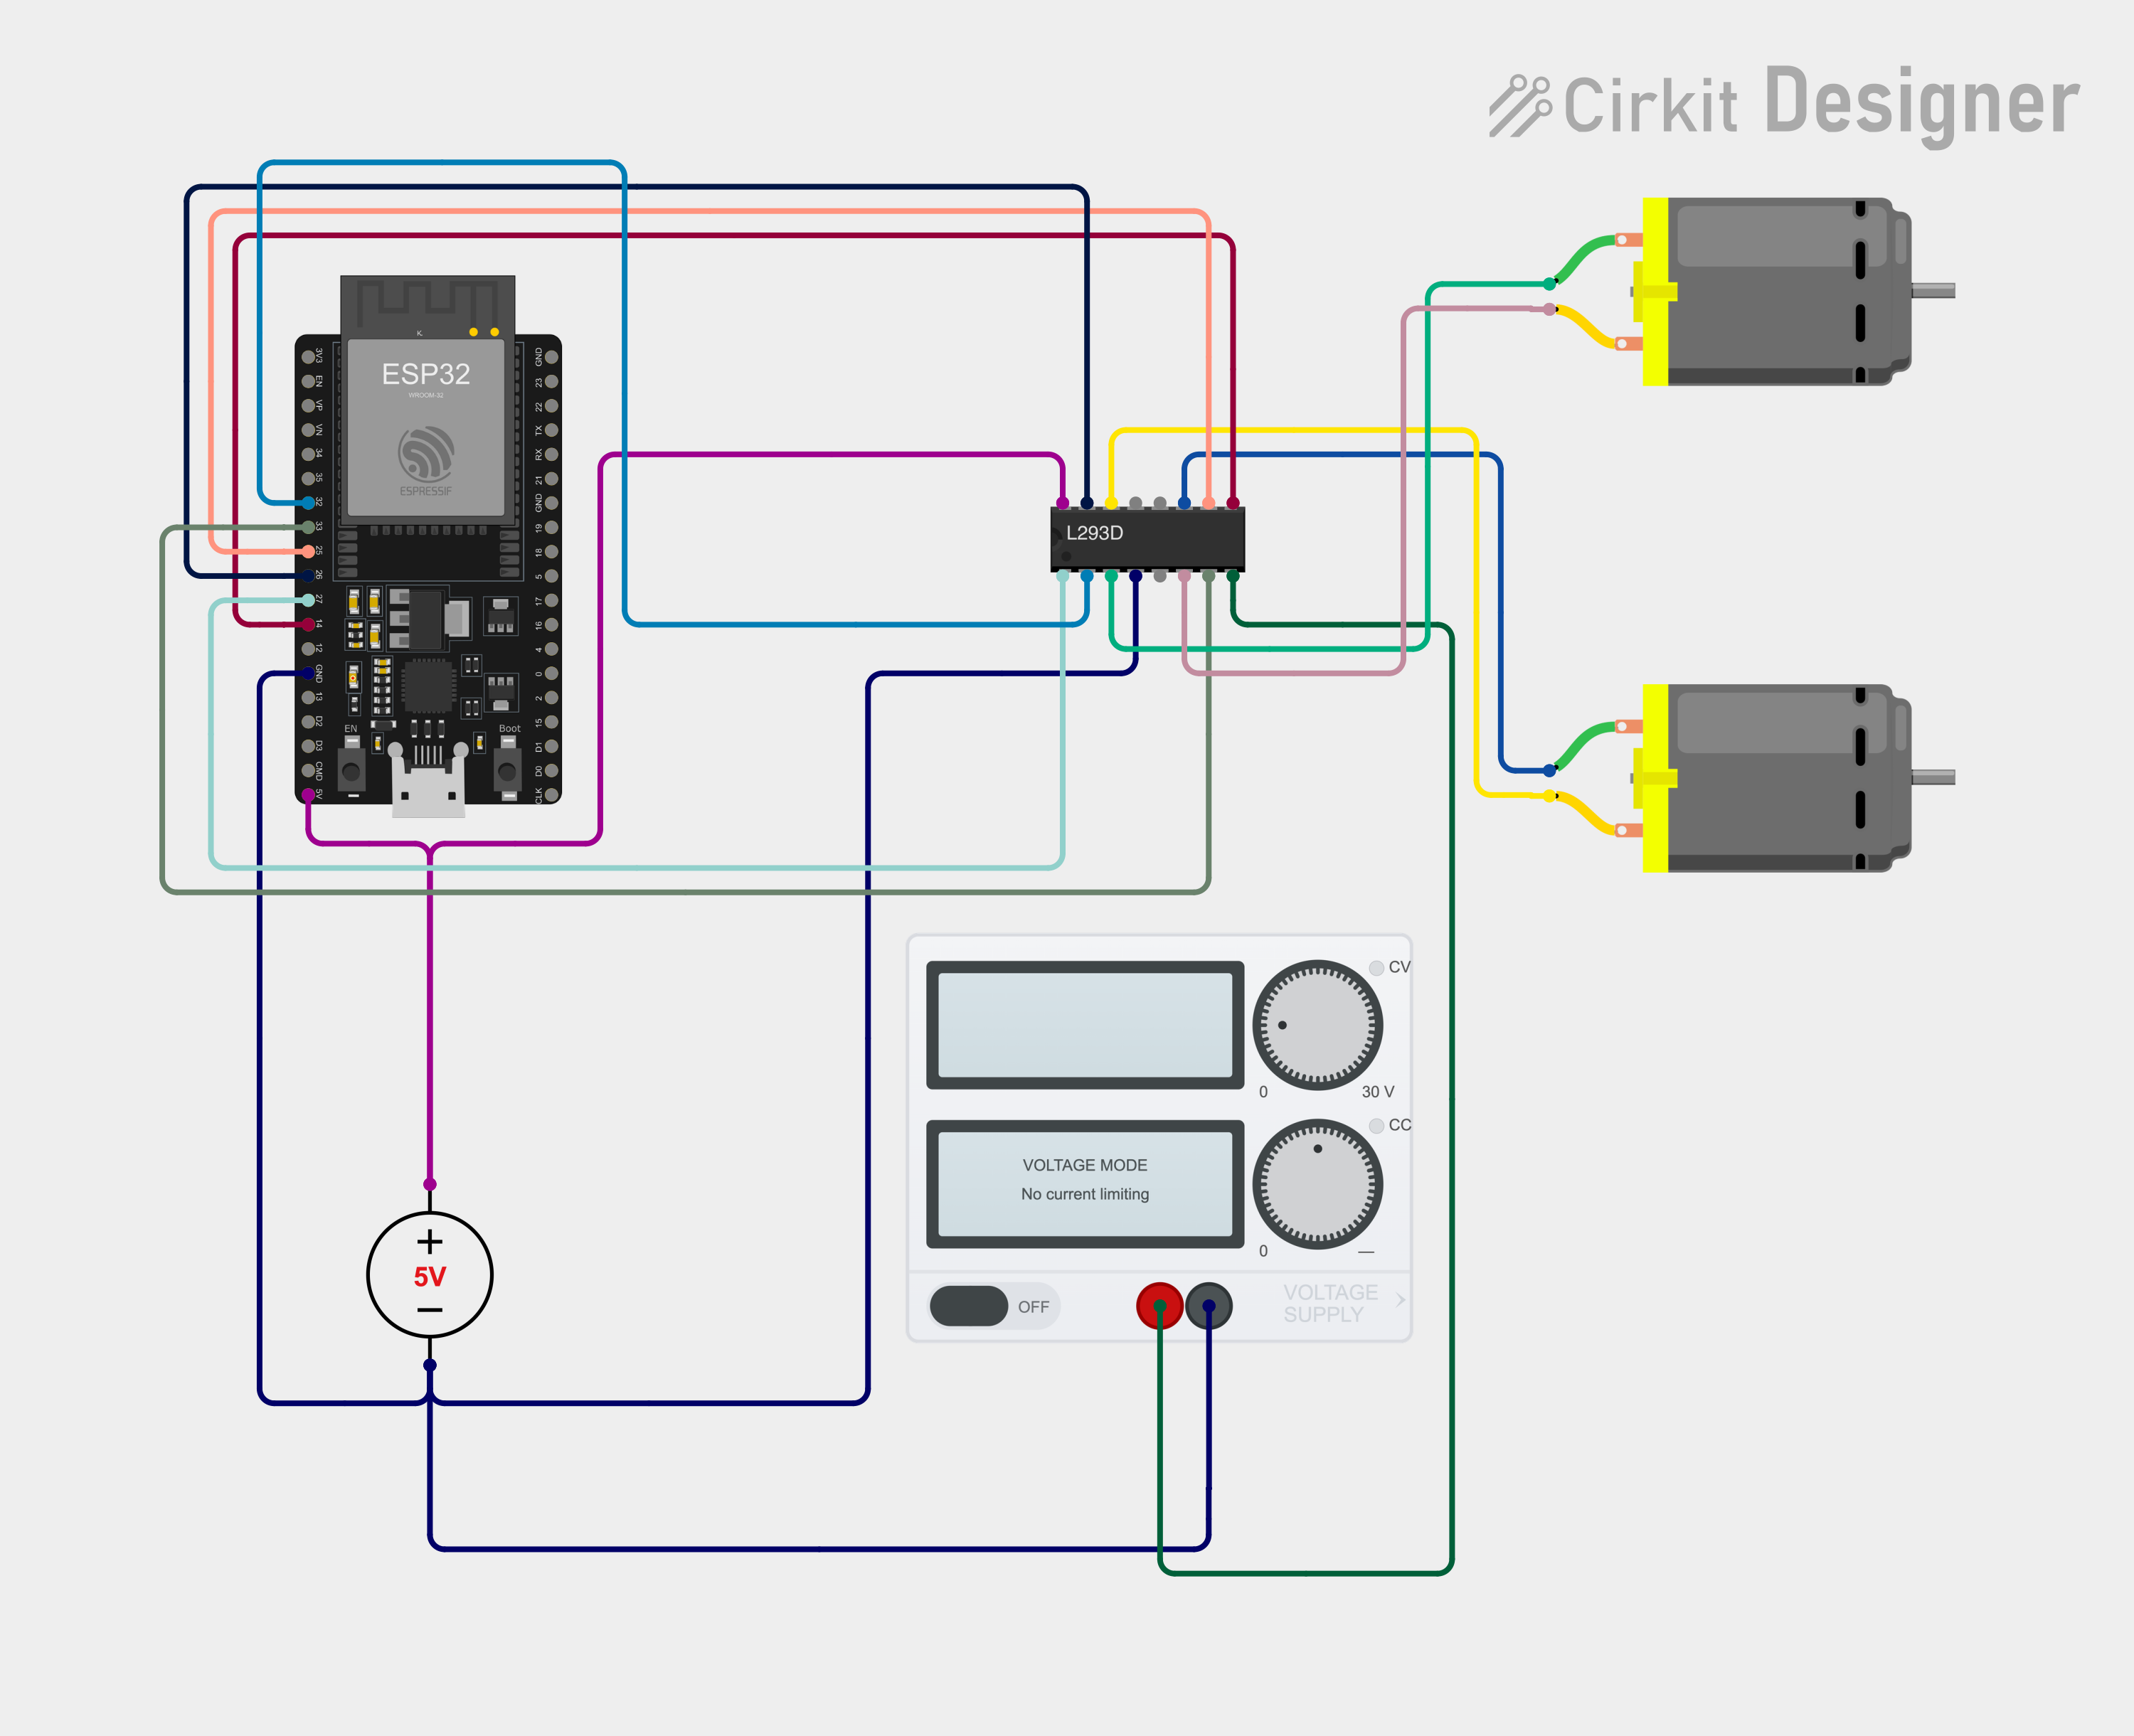
\includegraphics[width=0.70\linewidth,height=0.40\textheight,keepaspectratio]{bluetooth/esp32_bluetooth_circuit.png}
    \caption{ESP32 Bluetooth/Dabble model circuit diagram.}
    \label{fig:bluetooth-circuit}
\end{figure}


\subsubsection{Differential-drive control}

The rover uses a differential-drive arrangement.
The two motors can be controlled independently,
allowing the vehicle to move forward, reverse,
or turn.

The firmware combines the horizontal and vertical
control requests using:

\[
L_{\mathrm{raw}}=y+x
\]

\[
R_{\mathrm{raw}}=y-x
\]

Here, \(L_{\mathrm{raw}}\) and \(R_{\mathrm{raw}}\)
represent the left and right motor requests before
normalisation.

For forward motion, both motors receive commands
in the forward direction. For reverse motion,
both receive reverse commands.

When a steering input is combined with forward
or reverse movement, the two motor commands become
different, producing a turning motion.

If either calculated value exceeds the allowed
range, the firmware normalises the pair to keep
the motor commands within the permitted limits.


\subsubsection{PWM speed control}

The firmware uses PWM to control the effective
drive supplied to the motors.

The configured PWM parameters are:

\begin{itemize}
    \item PWM frequency: 5 kHz.
    \item Resolution: 8 bits.
    \item PWM range: 0--255.
    \item Initial speed level: 5.
    \item Available speed levels: 3--7.
    \item Minimum non-zero PWM value: 90.
    \item Maximum PWM value: 255.
\end{itemize}

The Triangle button increases the selected speed
level, while the Cross button decreases it.

The minimum non-zero PWM value helps the motors
overcome their starting friction. Actual speed
also depends on the motor, battery condition,
mechanical load, and surface.


\subsubsection{Model photographs and demonstration}

\begin{figure}[H]
    \centering
    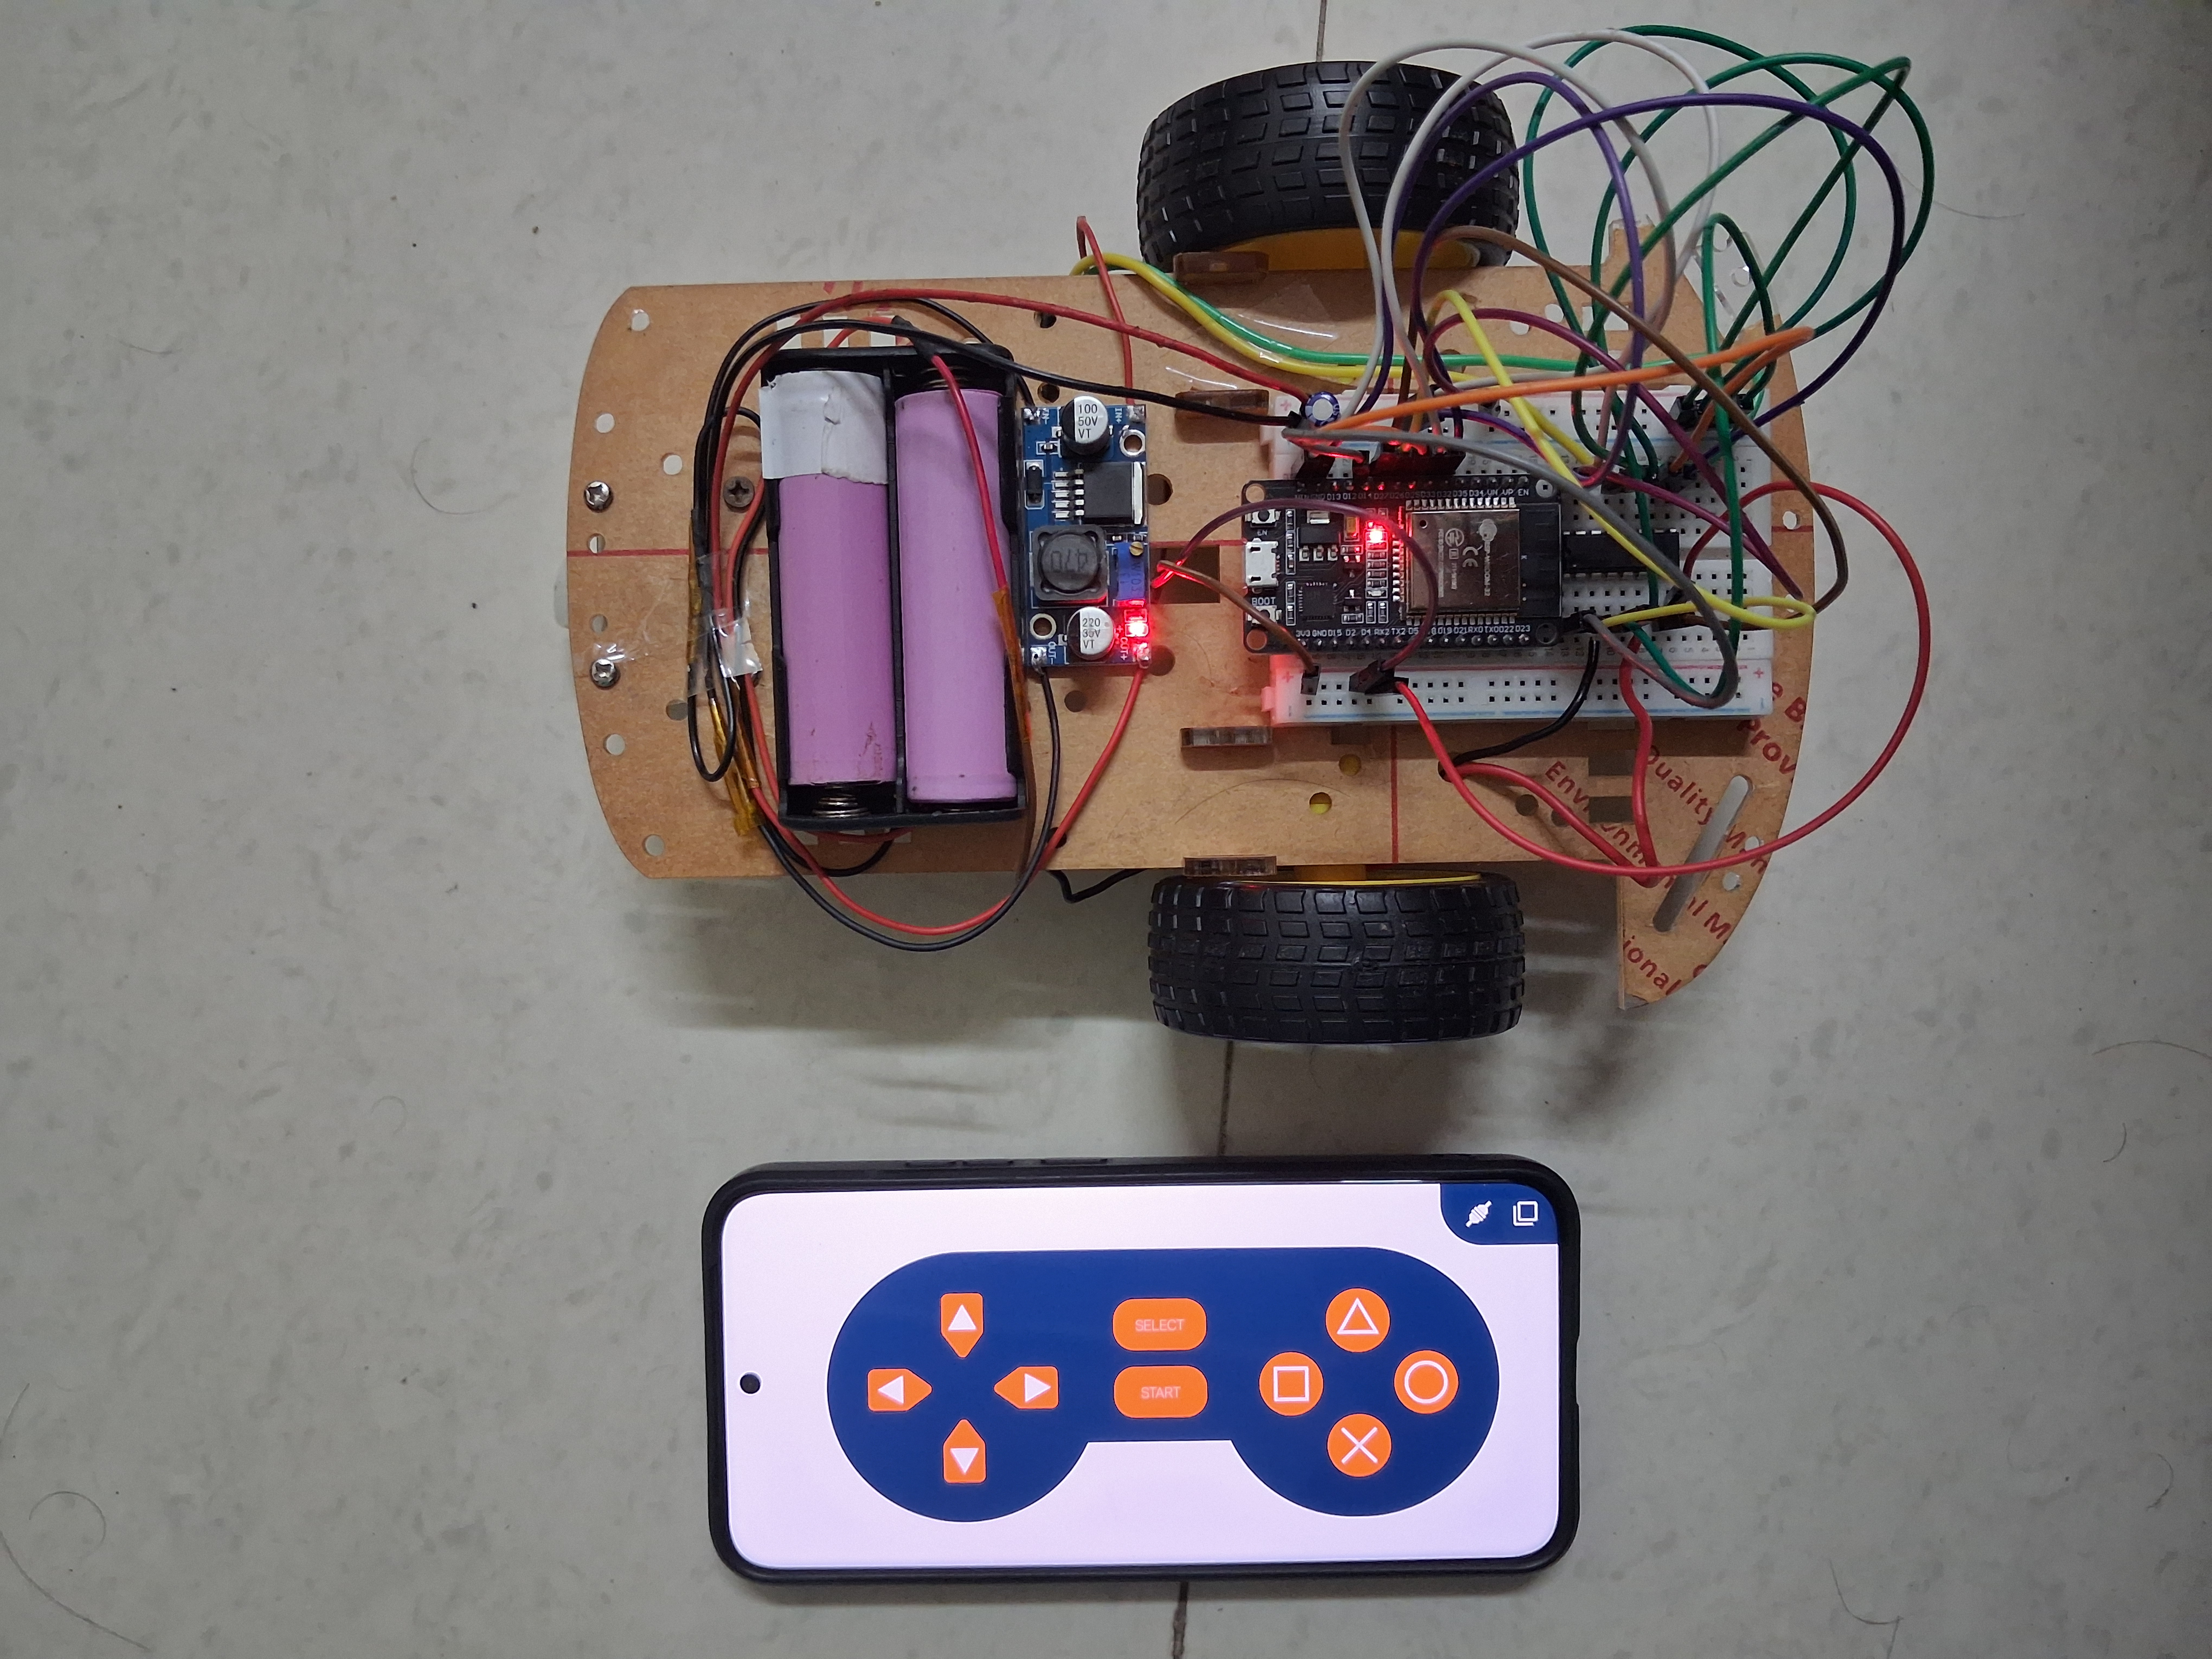
\includegraphics[width=0.70\linewidth,height=0.40\textheight,keepaspectratio]{bluetooth/bluetooth_rover.jpg}
    \caption{Assembled Bluetooth-controlled rover.}
    \label{fig:bluetooth-rover}
\end{figure}


\subsubsection{Source code and demonstration}

The complete firmware is maintained separately
from this report.

\textbf{Source-code path:}

\codepath{codes/bluetooth/main.ino}

\textbf{Circuit diagram link:}

\href{https://app.cirkitdesigner.com/project/77bb9468-2125-4b6d-bb11-cdf86b1c76d2}{Open ESP32 Bluetooth/Dabble circuit in Cirkit Designer}

\textbf{Demonstration video:}

\href{https://youtube.com/shorts/E_w3tyV0lKo?feature=share}{Watch Bluetooth/Dabble rover demonstration}


\subsubsection{Model outcome}

The Bluetooth model established the initial wireless
motor-control approach. The ESP32 DevKit communicated
with the Dabble application and used the received
inputs to control the two motors.

The implementation introduced the basic control
functions required by the later models: direction
selection, differential-drive calculation, PWM
speed control, and motor inversion.


% =================================================
% MODEL 2: LOCAL WI-FI
% =================================================

\newpage

\subsection{Model 2: Local Wi-Fi Joystick Control Using Raspberry Pi Pico W}
\label{model:wifi}

\subsubsection{Objective and system overview}

The second model was developed to provide wireless
control through a browser-based joystick interface.

A Raspberry Pi Pico W acts as both the controller
and the local Wi-Fi access point. A phone or laptop
connects directly to the network created by the
Pico W and opens the control webpage in a browser.

The webpage sends joystick coordinates to the
controller using HTTP requests. The Pico W processes
these values and generates the corresponding
motor commands.

This approach avoids the need for a separate
mobile application and allows the control interface
to be accessed through a standard browser.


\subsubsection{Local Wi-Fi access point}

The Pico W creates a wireless access point with
the SSID:

\begin{center}
    \texttt{UGV}
\end{center}

The phone or laptop connects directly to this
network.

The Pico W runs an HTTP server on port 80.
After connecting to the access point, the user
opens the following address in the browser:

\begin{center}
    \texttt{http://192.168.4.1}
\end{center}

This is a local network connection. It does not
require an external router or an internet connection.


\subsubsection{Multi-device access and simultaneous connectivity}

A major feature of this architecture is its ability
to support multiple connected devices.

The Raspberry Pi Pico W supports up to
\textbf{4 simultaneous Wi-Fi clients} in access-point
mode. This means that up to four phones or laptops
can connect to the same \texttt{UGV} wireless network
at the same time.

Each connected device can independently open the
browser-based control webpage using the local
IP address.

This makes the system useful in situations where
more than one person needs access to the rover's
interface.

For example, one device can be used to operate
the joystick while other connected devices can
open the same interface to observe the control
page and the system's response.

The multi-device architecture provides the following
advantages:

\begin{itemize}

    \item \textbf{Multiple client connections:}
    Up to four devices can connect to the rover's
    access point simultaneously.

    \item \textbf{Shared browser interface:}
    Each connected device can access the same
    control webpage without installing a dedicated
    application.

    \item \textbf{Flexible access:}
    Different phones and laptops can connect
    to the rover using the same local network.

    \item \textbf{No external router required:}
    The Pico W itself creates the network, making
    the system self-contained.

    \item \textbf{Local operation:}
    Devices can access the rover even when an
    internet connection is unavailable.

\end{itemize}

The four-client limit is the maximum supported
simultaneous access-point connection count, not
a guarantee of identical performance for every
connected device.

All devices communicate with the same controller
and therefore share the same motor outputs.
If multiple devices issue movement commands,
the controller processes the received requests
as they arrive. A later command may override
an earlier movement command.

Thus, the system provides simultaneous multi-device
access and shared control, rather than four
independent motor-control channels.

The four-client capability is specified in the
Raspberry Pi Pico W wireless documentation and
the Arduino-Pico Wi-Fi documentation.


\subsubsection{Browser-based joystick interface}

The webpage contains a virtual joystick that can
be operated using a touchscreen or a mouse.

The joystick provides two normalised values:

\[
-1 \leq x \leq 1
\]

\[
-1 \leq y \leq 1
\]

The horizontal coordinate \(x\) represents steering,
while the vertical coordinate \(y\) represents
forward and reverse movement.

The interface also provides a STOP button.

\begin{figure}[H]
    \centering
    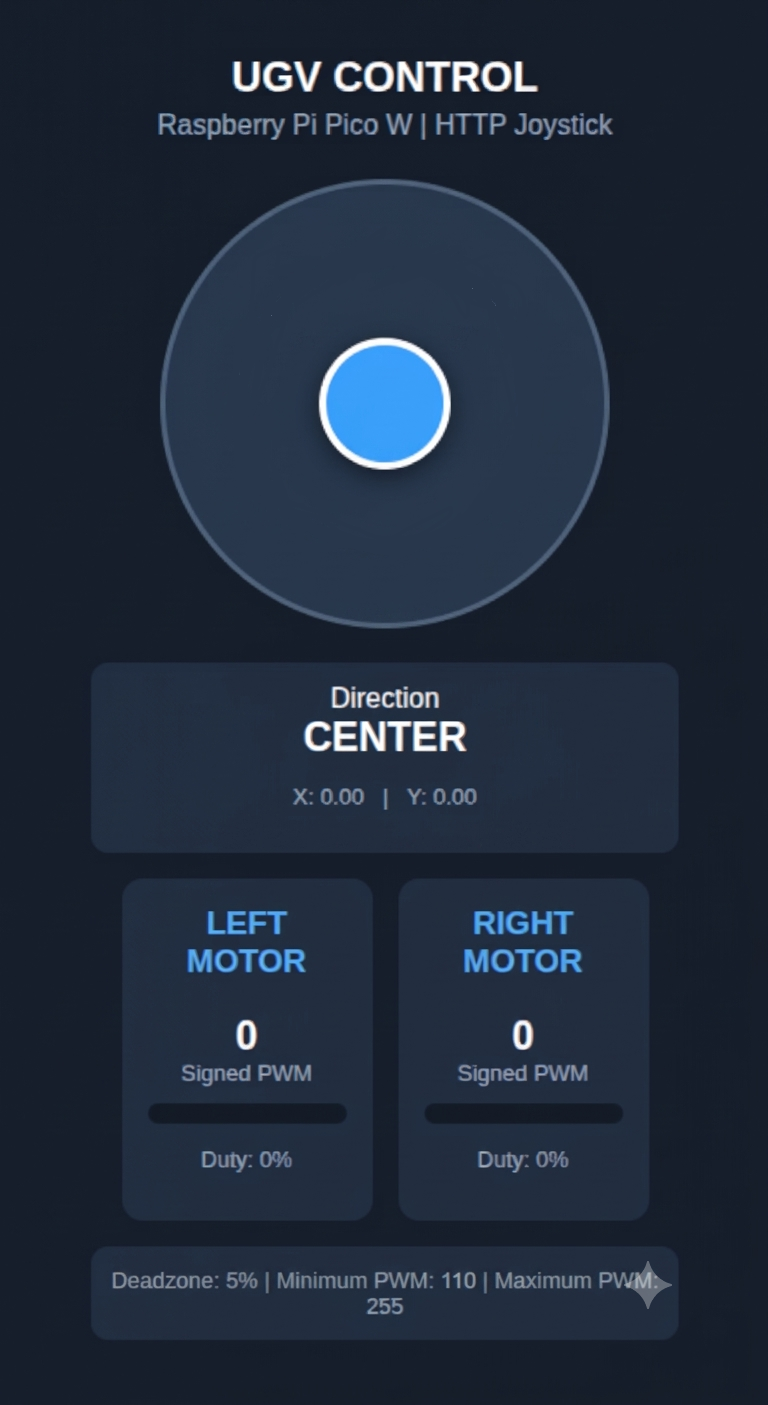
\includegraphics[width=0.70\linewidth,height=0.40\textheight,keepaspectratio]{pico_w/pico_wifi_joystick.png}
    \caption{Browser-based local Wi-Fi joystick interface.}
    \label{fig:pico-w-joystick}
\end{figure}


\subsubsection{HTTP communication}

The browser communicates with the Pico W through
HTTP requests.

When the joystick is moved, the webpage sends
the horizontal and vertical values through a
request following this general format:

\begin{center}
    \texttt{/drive?x=VALUE\&y=VALUE}
\end{center}

The controller reads the request, extracts the
two coordinates, and passes them to the motor-control
function.

A separate request is used to stop the rover:

\begin{center}
    \texttt{/stop}
\end{center}

The server returns a response after processing
the request.

The webpage and motor-control firmware therefore
operate as separate parts of the system. The
webpage supplies the requested movement, while
the Pico W calculates and applies the motor commands.


\subsubsection{Differential-drive joystick calculation}

The Pico W combines the joystick coordinates to
calculate the left and right motor commands.

The differential-drive equations are:

\[
L_{\mathrm{raw}}=y+x
\]

\[
R_{\mathrm{raw}}=y-x
\]

If either result exceeds the permitted range,
both values are normalised using the largest
absolute value:

\[
M=\max\left(
|L_{\mathrm{raw}}|,
|R_{\mathrm{raw}}|
\right)
\]

When \(M>1\), the values are divided by \(M\).

The resulting values are scaled to the PWM range.

The sign of each motor command determines its
direction, while its absolute value determines
the PWM magnitude.

This allows proportional steering. For example,
when the joystick is pushed forward while slightly
to the right, the two motors receive different
commands, producing a curved path.


\subsubsection{Dead zone and command updates}

A small dead zone is used around the centre of
the joystick to avoid unwanted movement caused
by minor touch-position changes.

The dead-zone threshold is:

\[
r < 0.05
\]

where:

\[
r=\sqrt{x^2+y^2}
\]

When the joystick radius is below the threshold,
the controller stops the motors.

The browser sends joystick updates every
20 milliseconds, corresponding to a nominal
update frequency of:

\[
f=\frac{1}{0.020}=50\text{ Hz}
\]

This update interval is intended to provide
responsive control while keeping the browser
and controller synchronised during movement.


\subsubsection{Motor connections and PWM}

The Pico W uses the following GPIO mapping
for the L293D motor driver.

\begin{center}
\begin{tabular}{lll}
\toprule
\textbf{Function}
&
\textbf{Pico W GPIO}
&
\textbf{Purpose}
\\
\midrule
Left enable / PWM & 10 & Left motor speed\\
Left direction 1 & 11 & Left motor direction\\
Left direction 2 & 12 & Left motor direction\\
Right direction 1 & 13 & Right motor direction\\
Right direction 2 & 14 & Right motor direction\\
Right enable / PWM & 15 & Right motor speed\\
\bottomrule
\end{tabular}
\end{center}

The right motor uses an inversion setting to
account for its physical orientation.

The PWM range is configured from 0 to 255,
with a frequency of 1000 Hz.

The practical starting threshold of the motors
is also important. A PWM command that is too
small may not overcome the motor's starting
friction.

A PWM value around 110 was identified as a
practical starting threshold during testing.
The exact minimum value should remain consistent
with the final firmware revision.


\subsubsection{Circuit diagram}
\label{subsec:pico-circuit}
\begin{figure}[H]
    \centering
    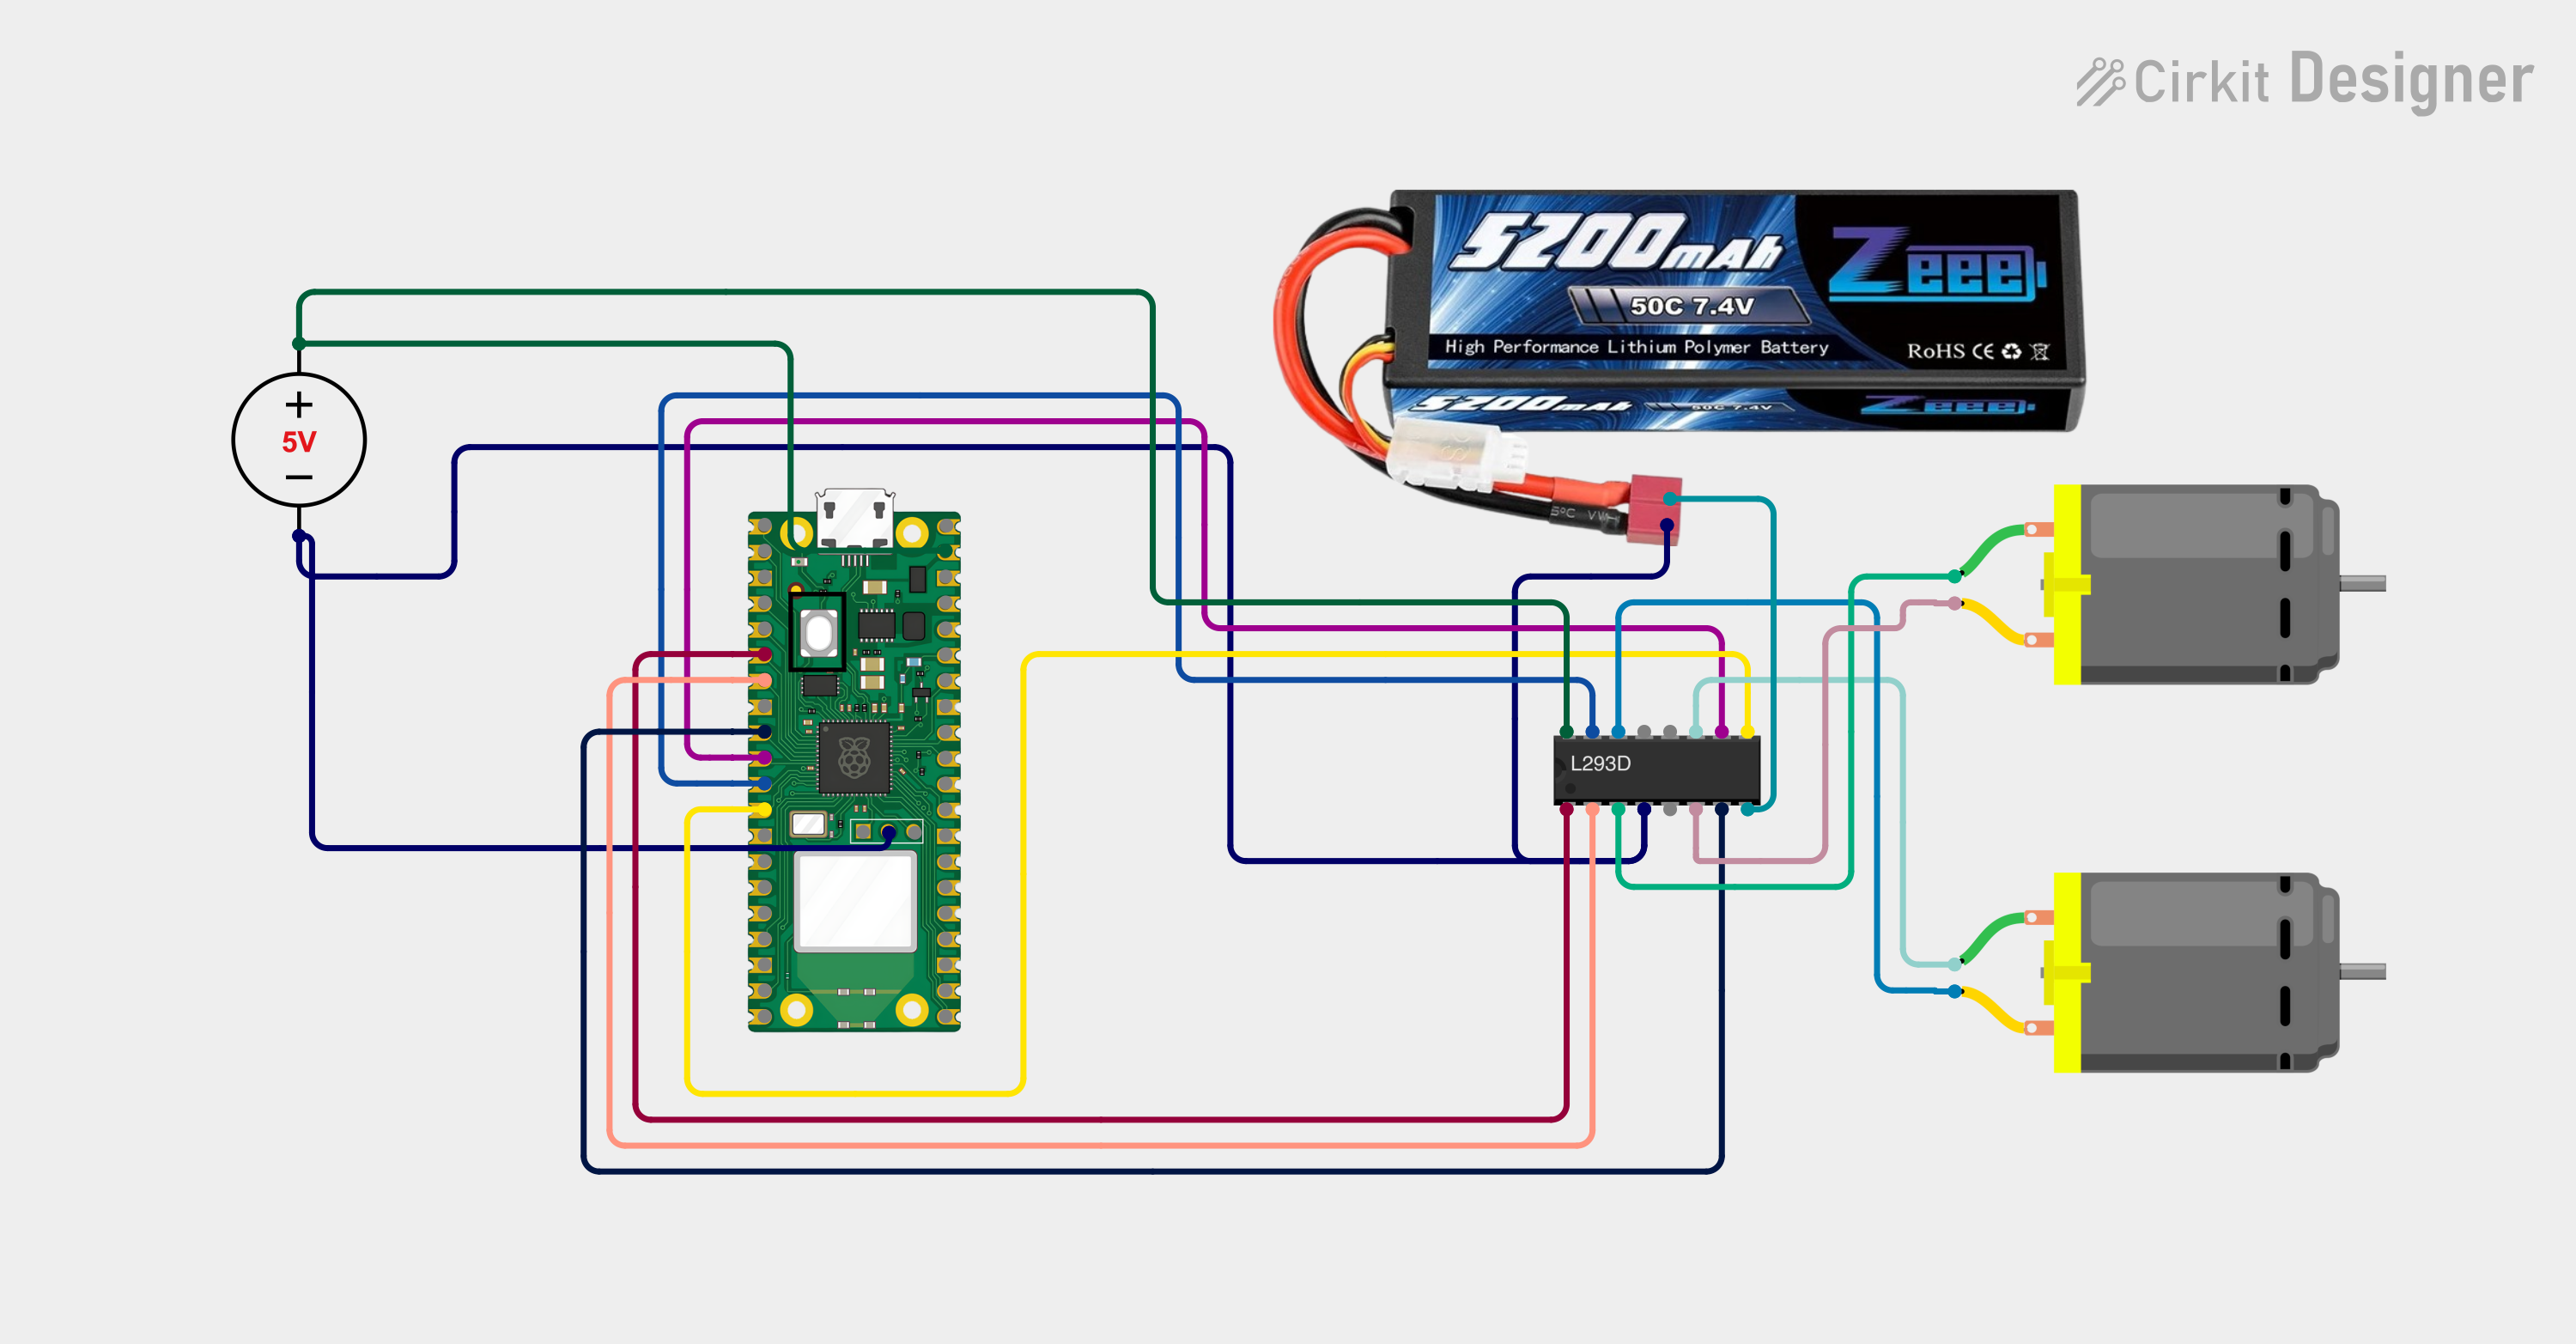
\includegraphics[width=0.70\linewidth,height=0.40\textheight,keepaspectratio]{pico_w/pico_w_circuit.png}
    \caption{Raspberry Pi Pico W and L293D circuit diagram.}
    \label{fig:pico-circuit}
\end{figure}


\subsubsection{Command timeout and stopping behaviour}

A remote-control system should not continue
moving indefinitely if the control connection
is interrupted.

The browser sends a stop request when the user
releases or cancels the joystick interaction.

The firmware also contains a watchdog mechanism.
If the controller does not receive a new movement
command within the configured timeout, it stops
the motors.

The watchdog timeout in the documented firmware is:

\[
T_{\mathrm{watchdog}}=250\text{ ms}
\]

The browser-side stop request is the normal
stopping mechanism. The watchdog provides a
backup if the browser stops sending updates
because of a connection interruption or another
unexpected event.

These two mechanisms serve different purposes
and work together to improve stopping reliability.


\subsubsection{Serial monitoring and telemetry}

The firmware provides serial output to help
observe the controller's response to joystick
inputs.

The telemetry includes:

\begin{itemize}
    \item Joystick X and Y coordinates.
    \item Joystick radius and direction.
    \item Left and right motor directions.
    \item Signed motor commands.
    \item PWM magnitudes and duty-cycle percentages.
    \item Watchdog state.
\end{itemize}

The serial monitor operates at 115200 baud.
This information is useful for observing the
internal control calculations and troubleshooting
the motor-control system.


\begin{figure}[H]
    \centering
    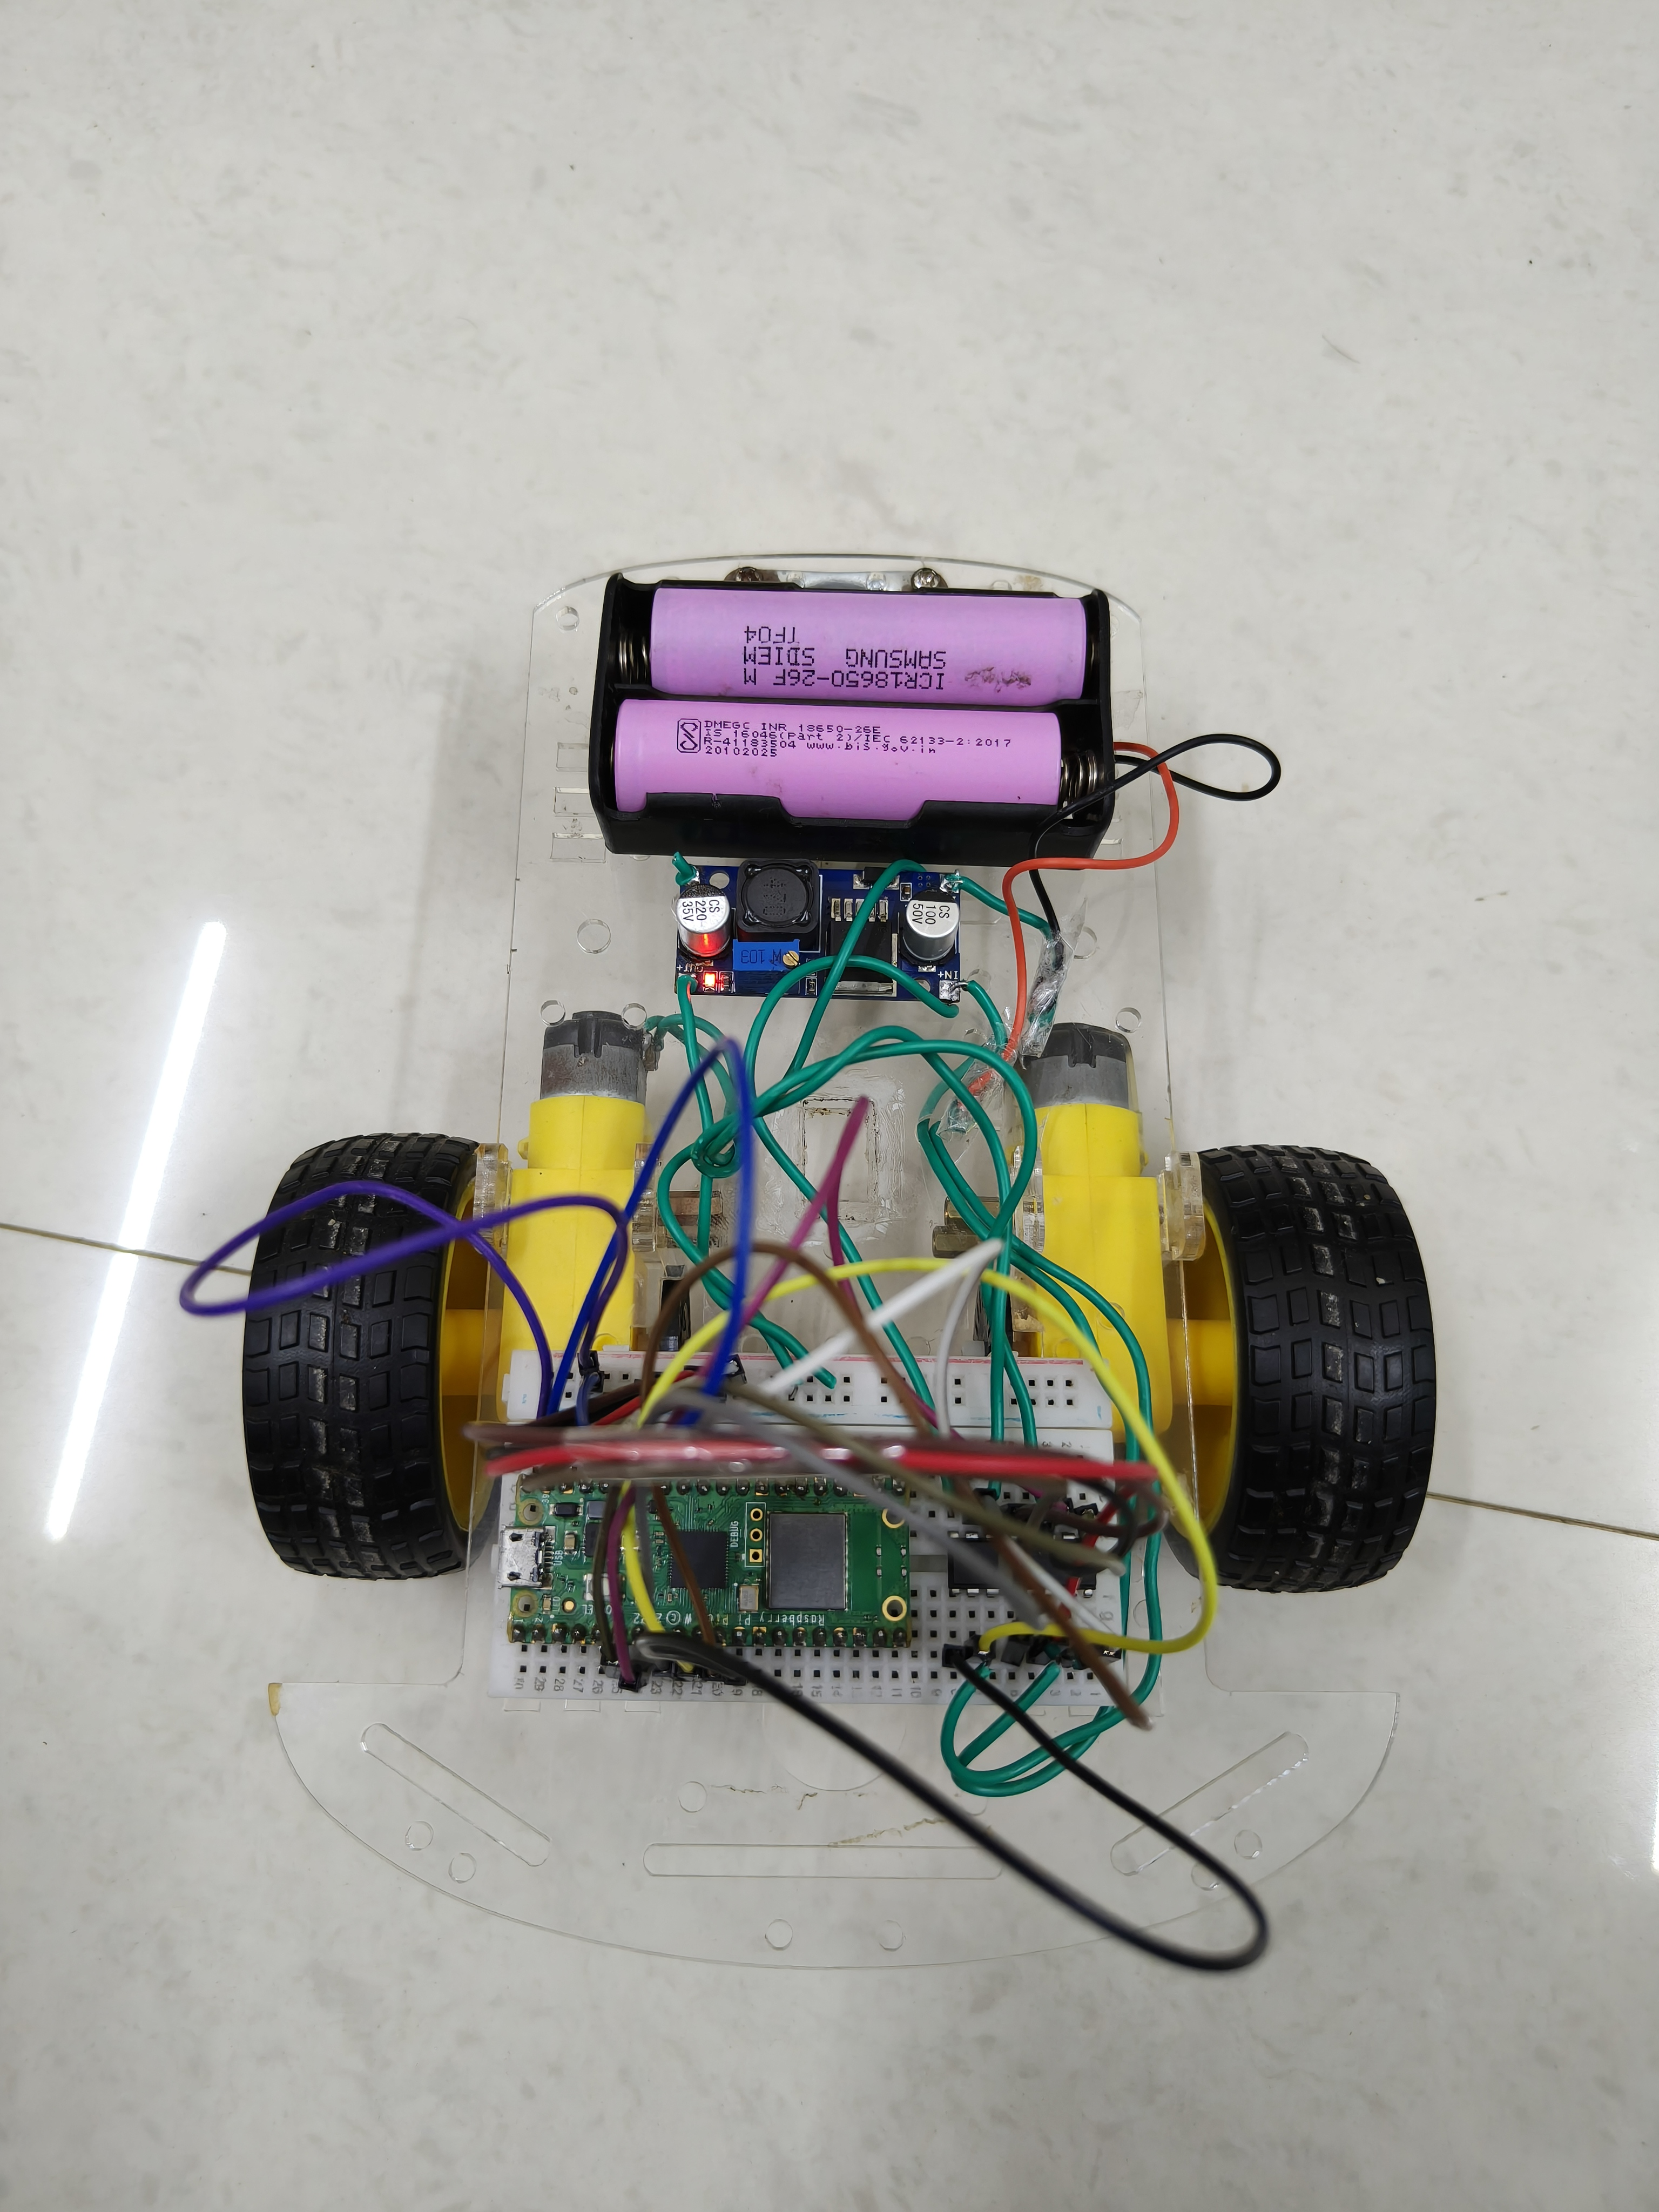
\includegraphics[width=0.70\linewidth,height=0.40\textheight,keepaspectratio]{pico_w/pico_w_rover.jpg}
    \caption{Assembled Raspberry Pi Pico W local Wi-Fi rover.}
    \label{fig:pico-w-rover}
\end{figure}


\subsubsection{Controller transition and design limitation}

The development of the local Wi-Fi model involved
a change of controller.

The ESP32 DevKit had worked properly in the initial
Bluetooth model. However, its later Wi-Fi operation
was not sufficiently reliable during testing.
We suspected that the power arrangement might
have contributed to the problem, but the exact
cause was not confirmed.

We then attempted to use a NodeMCU board, but
it did not work as expected for the intended
implementation.

We therefore moved to the Raspberry Pi Pico W
for the local Wi-Fi joystick model.

The Pico W successfully provided the local
access-point architecture required for
browser-based control.

However, this local access-point arrangement
is different from connecting directly to the
IITH campus network using WPA2-Enterprise
authentication.


\subsubsection{Model outcome}

The local Wi-Fi model established a browser-based
control approach using the Raspberry Pi Pico W.

Its main features include:

\begin{itemize}
    \item A local Wi-Fi access point named \texttt{UGV}.
    \item An HTTP server hosted by the Pico W.
    \item A browser-based joystick interface.
    \item Proportional differential-drive control.
    \item PWM-based motor speed control.
    \item Multi-device access for up to four clients.
    \item A STOP request and watchdog timeout.
    \item Serial telemetry for observing control values.
\end{itemize}

The model provides a flexible local control
architecture in which multiple devices can
connect to the same rover without requiring
an external router or internet connection.


\subsubsection{Source code and demonstration}

The complete firmware is maintained separately
from this report.

\textbf{Source-code path:}

\codepath{codes/wifi_pico_w/main.ino}

\textbf{Circuit diagram link:}

\href{https://app.cirkitdesigner.com/project/8634cb3d-05e7-47cd-89a1-715ecb20721b}{Open Raspberry Pi Pico W circuit in Cirkit Designer}

\textbf{Demonstration video:}

\href{https://www.youtube.com/watch?v=DtV5GhC6SQU}{Watch Pico W local Wi-Fi joystick demonstration}


% =================================================
% MODEL 3: ESP32-CAM
% =================================================

\newpage

\subsection{Model 3: ESP32-CAM Campus Camera Rover}
\label{model:camera}

\subsubsection{Objective and system overview}

The third model was intended to extend the rover's
capabilities by combining remote operation with
a camera-based view of its surroundings.

An ESP32-CAM board was used for this model.
The intended architecture involved connecting
the board to the IITH campus Wi-Fi network and
using the camera to provide a live video feed.

The operator would be able to access the rover
over the network and observe the camera feed
while issuing movement commands.


\subsubsection{Campus Wi-Fi connection}

The ESP32-CAM was successfully connected to
the IITH campus Wi-Fi network using WPA2-Enterprise
authentication.

This confirmed that the campus-network connection
could be established with the ESP32-CAM.

The remaining difficulty was associated with
the camera hardware and its interfacing.


\subsubsection{Camera interfacing}

The camera module was intended to provide a
live video stream from the rover.

However, during setup, we encountered a camera
hardware or interfacing problem that prevented
successful camera initialisation.

As a result, we could not complete the live-streaming
implementation or demonstrate the intended
combined camera and motor-control system.

The camera problem should be treated separately
from the campus Wi-Fi connection, since the
network connection itself was successfully
established.


\subsubsection{Circuit diagram}
\label{subsec:esp32cam-circuit}
\begin{figure}[H]
    \centering
    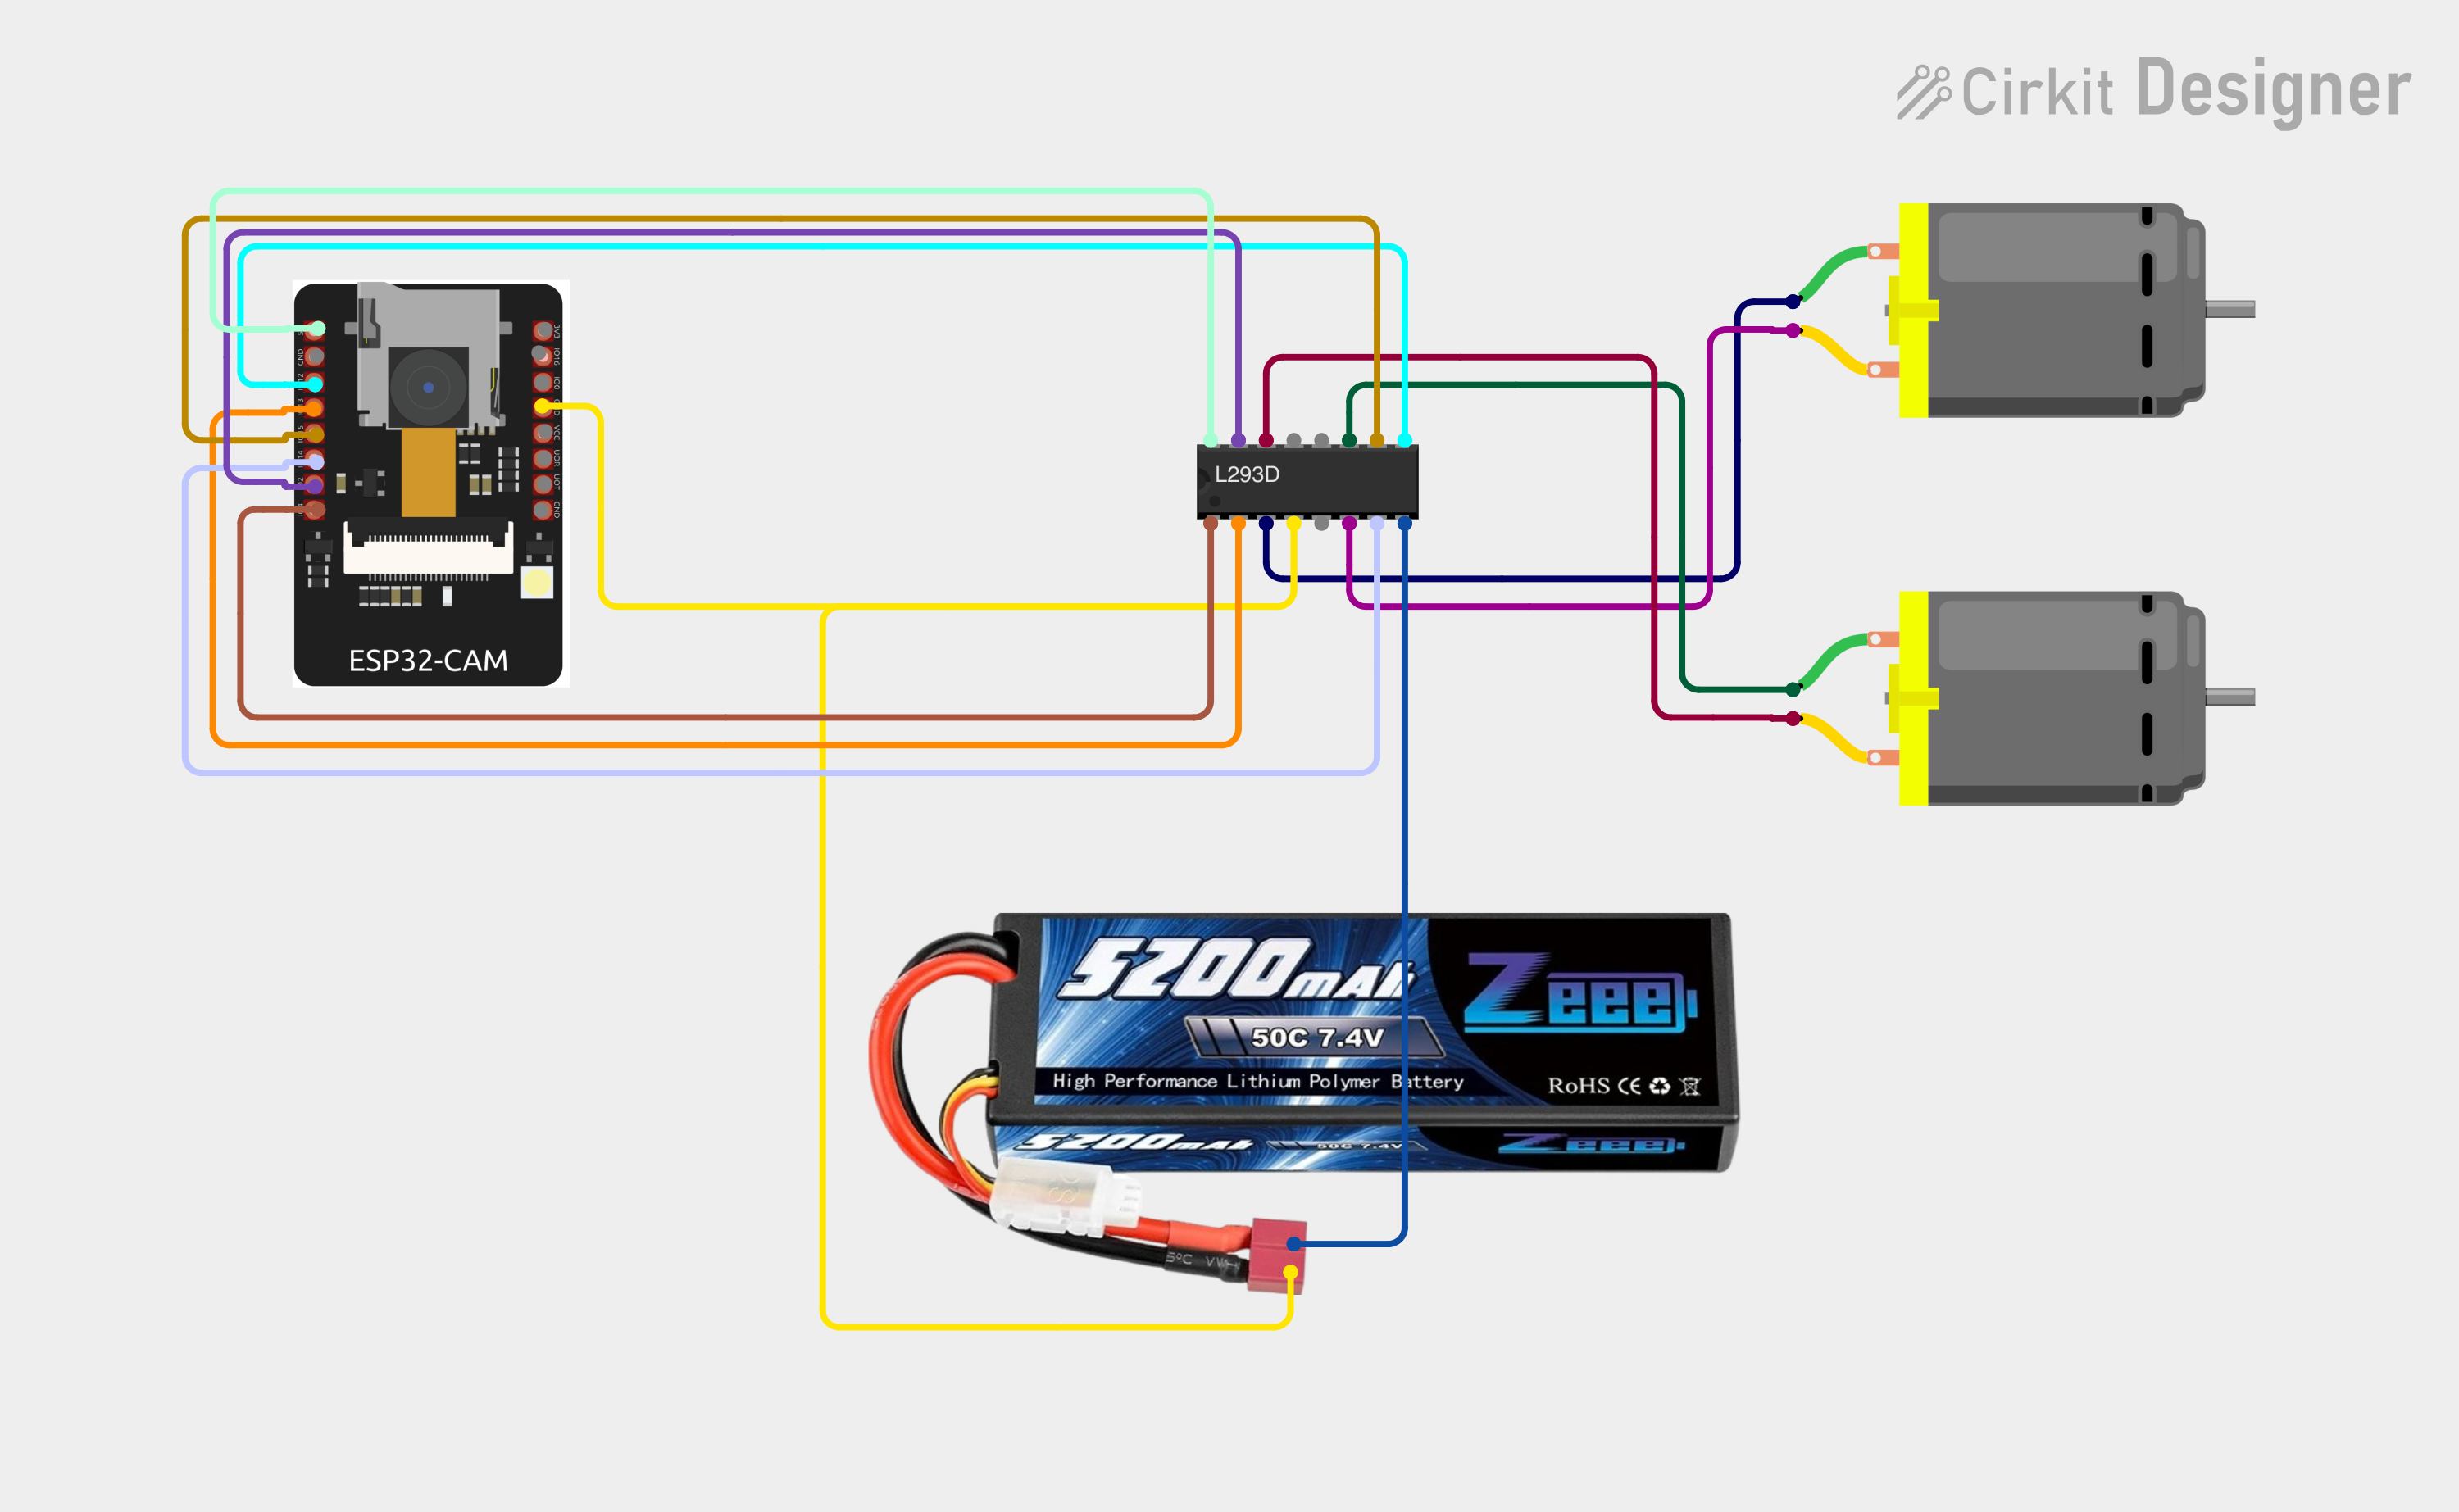
\includegraphics[width=0.70\linewidth,height=0.40\textheight,keepaspectratio]{esp32_cam/esp32_cam_circuit.png}
    \caption{ESP32-CAM rover circuit diagram.}
    \label{fig:esp32cam-circuit}
\end{figure}


\subsubsection{Prescribed motor-driver GPIO mapping}

The circuit reference specifies the following ESP32-CAM connections to the L293D:

\begin{center}
\begin{tabular}{lll}
\toprule
\textbf{Function} & \textbf{ESP32 GPIO} & \textbf{L293D pin}\\
\midrule
Left direction input 1 & 13 & 2\\
Left direction input 2 & 14 & 7\\
Right direction input 1 & 15 & 10\\
Right direction input 2 & 2 & 15\\
Left enable / PWM (EN1) & 4 & 1\\
Right enable / PWM (EN2) & 12 & 9\\
\bottomrule
\end{tabular}
\end{center}

The L293D logic supply connects to pin 16, while the motor supply connects separately to pin 8. All circuit grounds must be common. The motor battery positive must not be connected to the ESP32-CAM 5 V pin. This is the prescribed mapping from the circuit reference; its compatibility must be checked against the exact ESP32-CAM board and camera configuration because some GPIOs may be shared with camera, flash, or SD functions.


\subsubsection{Intended operation}

The intended operating sequence was:

\begin{enumerate}
    \item Power the ESP32-CAM and initialise the board.
    \item Connect the board to the IITH campus Wi-Fi
    network using WPA2-Enterprise authentication.
    \item Initialise the camera module.
    \item Start the camera server or streaming interface.
    \item Access the rover through an authorised device
    on the network.
    \item Use the camera feed to observe the surroundings
    while controlling the rover.
\end{enumerate}

The camera initialisation problem prevented
completion of this sequence.


\subsubsection{Further development}

The next step would be to verify the camera module
independently and confirm that it can initialise
successfully.

After that, the live video stream should be tested
separately from the motor-control system. Once
both the camera and network functions operate
reliably, they can be integrated into a single
remote-control interface.

Further testing should examine video delay,
connection stability, and the effect of motor
operation on the camera feed.





\subsubsection{Model outcome}

The ESP32-CAM model established the intended
direction for a campus-network-connected
camera rover.

The WPA2-Enterprise campus Wi-Fi connection
was successful. However, the camera interfacing
problem prevented completion of the live video
stream.

The model is therefore recorded as an attempted
implementation with an incomplete camera
subsystem. A successful live camera feed or
completed camera-based remote-control
demonstration is not claimed.


\subsubsection{Source code and demonstration}

The camera firmware is maintained separately
from this report.

\textbf{Source-code path:}

\codepath{codes/esp32_cam/main.ino}

\textbf{Circuit diagram link:}

\href{https://app.cirkitdesigner.com/project/1818aafd-fd66-4861-99ec-7fd3e9db77a6}{Open ESP32-CAM rover circuit in Cirkit Designer}

No demonstration video is included because a successful camera-streaming demonstration was not completed.


% =================================================
% RESEARCH MODELS
% =================================================

\newpage

\subsection{Research Models}
\label{sec:research-models}

\subsubsection{Dynamic Node Hopping}

\textbf{Research objective}

Dynamic Node Hopping explores a possible way to
extend the communication range of the UGV by
using intermediate wireless relay nodes.

In a direct communication system, the operator's
device communicates with the rover through a
single wireless link. The useful range is
therefore limited by the quality and availability
of that connection.

Dynamic Node Hopping proposes intermediate nodes
that forward commands and telemetry between the
operator and the rover.


\subsubsection{Proposed architecture}

The proposed arrangement consists of three
main elements:

\begin{itemize}

    \item \textbf{Operator node:}
    The phone or computer used to issue movement
    commands and receive information from the rover.

    \item \textbf{Intermediate relay nodes:}
    Wireless nodes that receive and forward packets
    between other nodes.

    \item \textbf{UGV node:}
    The final node that receives movement commands
    and sends telemetry back through the network.

\end{itemize}

A simplified communication path is:

\[
\text{Operator}
\longrightarrow
\text{Relay 1}
\longrightarrow
\text{Relay 2}
\longrightarrow
\text{UGV}
\]


\begin{figure}[H]
    \centering
    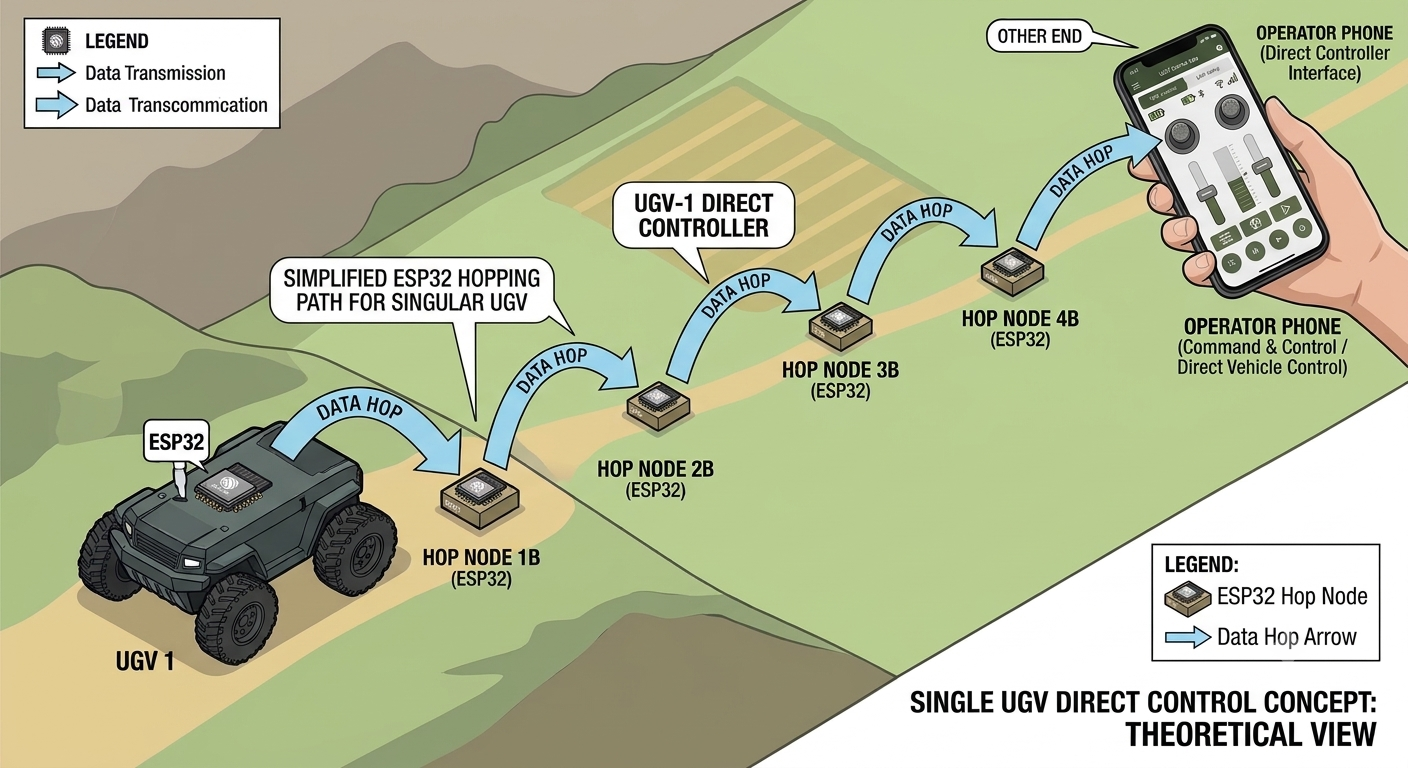
\includegraphics[width=0.70\linewidth,height=0.40\textheight,keepaspectratio]{hopping/dynamic_node_hopping.png}
    \caption{Proposed Dynamic Node Hopping architecture.}
    \label{fig:dynamic-node-hopping}
\end{figure}


\subsubsection{Dynamic route selection}

A key part of the concept is the ability to select
a suitable communication route.

If the rover moves away from one relay node or
a wireless connection becomes weak, the system
could attempt to select another available path.

Possible factors for route selection include:

\begin{itemize}
    \item Signal quality between neighbouring nodes.
    \item Communication delay.
    \item Packet loss.
    \item Availability of relay nodes.
    \item Number of hops required to reach the rover.
\end{itemize}

A route with more relay nodes may extend the
communication range, but it can also introduce
additional delay.


\subsubsection{Communication reliability and safe stopping}

Remote motor control requires predictable
communication.

If a relay node becomes unavailable, the system
must detect the communication failure and respond
appropriately.

The proposed design should include:

\begin{itemize}
    \item Detection of missing or failed relay links.
    \item Monitoring of packet delivery and delay.
    \item Route recovery when an alternative path exists.
    \item A timeout mechanism for missing control commands.
    \item A safe stop condition when communication is lost.
\end{itemize}


\subsubsection{Future research and testing}

The concept requires further investigation before
a physical implementation can be claimed.

Some of the questions to be studied are:

\begin{enumerate}
    \item How should relay nodes discover neighbouring nodes?
    \item How should the system select a route to the rover?
    \item How much delay is introduced by each additional hop?
    \item How does packet loss affect joystick control?
    \item How quickly can the network recover after a relay
    node becomes unavailable?
    \item How reliably can the rover stop when the
    communication path is interrupted?
\end{enumerate}

A future experimental setup could measure packet
loss, command delay, route recovery time, and
stopping response under different network conditions.


\subsubsection{Research status}

Dynamic Node Hopping is a proposed research
direction for extending the communication range
of the UGV.

A complete multi-node firmware system and physical
relay network were not implemented or tested
during the work recorded in this document.

No measured range improvement, packet-loss result,
or routing performance is therefore claimed.

The concept remains a possible future extension
of the wireless control system.


% =================================================
% CONCLUSION
% =================================================

\newpage

\section{Conclusion}

The project explored different approaches to
wireless control and remote operation of an
Unmanned Ground Vehicle.

The first model used an ESP32 DevKit with Bluetooth
communication through the Dabble application.
This provided the initial working approach for
wireless motor control.

The second model used a Raspberry Pi Pico W to
create a local Wi-Fi access point and host a
browser-based joystick interface. It introduced
HTTP communication, proportional joystick control,
differential-drive calculations, and watchdog-based
stopping behaviour. Its access-point architecture
also supports up to four connected Wi-Fi clients
simultaneously.

The third model explored a camera-assisted rover
using an ESP32-CAM connected to the IITH campus
Wi-Fi network. The WPA2-Enterprise connection
was successful, but a camera interfacing problem
prevented completion of the live video stream.

Finally, Dynamic Node Hopping was identified as
a possible research direction for extending the
communication range through intermediate relay
nodes. It remains a conceptual proposal rather
than a completed implementation.

The practical work highlighted the importance
of reliable wiring, suitable power arrangements,
correct motor-driver connections, and dependable
communication between the operator and the rover.


% =================================================
% END DOCUMENT
% =================================================

\end{document}
